\documentclass[11pt,letterpaper]{article}
\usepackage{fontspec}
\setmainfont{texgyrepagella}[Extension=.otf,UprightFont=*-regular,BoldFont=*-bold,ItalicFont=*-italic,BoldItalicFont=*-bolditalic]
\usepackage[bidi=default]{babel}
\babelprovide[import,main]{spanish}
\babelprovide[import]{hebrew}
\babelprovide[import]{ancientgreek}
\babelfont[hebrew]{rm}[Path=fonts/,BoldFont=NotoHebrewSerif-700.ttf,Scale=0.95]{NotoHebrewSerif-400.ttf}
\babelfont[ancientgreek]{rm}[Path=fonts/]{GFSPorson.otf}
\newcommand{\heb}[1]{\mbox{\foreignlanguage{hebrew}{#1}}}
\newcommand{\grc}[1]{\foreignlanguage{ancientgreek}{#1}}
\newcommand{\hebverso}[1]{\par\smallskip{\centering\begin{otherlanguage}{hebrew}\large #1\end{otherlanguage}\par}\smallskip}
\newcommand{\SENOR}{\textsc{Señor}}
\usepackage[margin=2.5cm,headheight=14pt]{geometry}
\usepackage{microtype,ragged2e,booktabs,graphicx,xcolor,csquotes,array}
\usepackage[hidelinks]{hyperref}\usepackage{xurl}\urlstyle{same}
\usepackage[most]{tcolorbox}
\usepackage{tikz}\usetikzlibrary{arrows.meta,positioning,calc,decorations.pathreplacing}
\usepackage{titlesec,fancyhdr}
\definecolor{azul}{HTML}{15437C}\definecolor{azuloscuro}{HTML}{0B1F3A}\definecolor{celeste}{HTML}{5694D6}
\definecolor{dorado}{RGB}{196,154,60}\definecolor{papiro}{RGB}{246,239,220}\definecolor{gris}{RGB}{70,78,96}
\titleformat{\section}{\Large\bfseries\color{azul}}{\thesection.}{0.6em}{}
\titleformat{\subsection}{\large\bfseries\color{azuloscuro}}{\thesubsection}{0.6em}{}
\pagestyle{fancy}\fancyhf{}
\fancyhead[L]{\foreignlanguage{spanish}{\small\itshape\color{gris}El Dios de todo saber}}\fancyhead[R]{\foreignlanguage{spanish}{\small\color{gris}\thepage}}
\renewcommand{\headrulewidth}{0.4pt}
\setlength{\parindent}{1.27cm}\linespread{1.15}\setlength{\emergencystretch}{3em}
\newtcolorbox{cita}[1][]{enhanced,colback=azul!6!white,colframe=azul,boxrule=0pt,leftrule=2.5pt,arc=0pt,
  left=8pt,right=8pt,top=5pt,bottom=5pt,before skip=8pt,after skip=8pt,fontupper=\itshape,#1}
\newcommand{\fuente}[1]{\par\hfill{\upshape\bfseries\small\textcolor{azul}{#1}}}
\newtcolorbox{nota}[1][]{enhanced,colback=dorado!10,colframe=dorado!85!azul,boxrule=0.6pt,arc=2pt,
  fonttitle=\bfseries\small,coltitle=azuloscuro,colbacktitle=dorado!30,fontupper=\small,title={#1}}
\newtcolorbox{filologia}[1][]{enhanced,colback=white,colframe=azul!45,boxrule=0.5pt,arc=2pt,
  fonttitle=\bfseries\small,coltitle=white,colbacktitle=azul!80,fontupper=\small,title={Filología: #1}}
\newcommand{\refapa}[1]{\par{\RaggedRight\hangindent=1.27cm\hangafter=1\noindent #1\par}\vspace{4pt}}
\newcommand{\destacar}[1]{\textbf{\textcolor{azul}{#1}}}
\newcolumntype{L}[1]{>{\RaggedRight\arraybackslash}p{#1}}

\title{\color{azul}\bfseries El Dios de todo saber\\[4pt]\large\color{gris}\mdseries La omnisciencia y la presciencia de Dios\\[2pt]``Oh \SENOR{}, tú me has examinado y conocido'' (Sal 139:1)}
\author{}\date{}
\begin{document}
\maketitle\thispagestyle{empty}

\begin{abstract}\noindent
Este capítulo estudia la omnisciencia de Dios y, como una particularidad de ella, su presciencia. Parte de dos definiciones: Dios lo conoce todo (lo real y lo posible, el pasado y el futuro, y el corazón), y la presciencia es su conocimiento-amor previo y soberano hacia sus escogidos. El texto ancla es el Salmo 139, leído en sus cuatro estrofas y en su hebreo; lo acompaña una sección expositiva sobre los Salmos que confiesan al Dios que ve, escudriña y cuenta (Sal 1; 7; 11; 17; 33; 38; 44; 56; 69; 90; 94; 103; 105; 113; 147), con el Salmo 113, el Dios que ``se humilla a mirar'', leído junto al cántico de Ana, que llama al \SENOR{} \emph{El deot}, ``el Dios de todo saber'' (1 S 2:3). La filología muestra que el verbo \emph{yadá} no es solo tener información: es conocer de cerca, con favor, y por eso puede significar escoger (Gn 18:19; Am 3:2). Se presenta el espectro de términos hebreos y griegos y el Nombre que revela el atributo: \emph{El roí}, ``el Dios que me ve, que Agar invoca en el desierto (Gn 16:13), junto con \emph{El deot}, con su eco en ``tu Padre que ve en lo secreto (Mt 6:6) y en el ser ``conocidos por Dios. Siguen una exposición teológica del atributo (nada se le oculta, conoce nuestra condición, saber no es decretar, la presciencia tiene personas por objeto) en diálogo con la tradición, las preguntas que plantean textos como ``ya conozco'' (Gn 22:12), un encuentro en la historia de Israel (``y los reconoció Dios'', Éx 2:25), la mirada judía (\emph{Avot} 3:15, la Misná de Rosh Hashaná, el midrash, Rashi, Maimónides y Qumrán) y la lectura de Pablo y de Pedro: la doxología de Romanos 11, la cadena de Romanos 8, ``conocidos por Dios'' (1 Co 8:3; Gá 4:9), los tesoros del conocimiento en Cristo (Col 2:3) y la presciencia en los discursos y cartas de Pedro (Hch 2:23; 1 P 1:2, 20), que la prueba con los Salmos dichos de antemano por el Espíritu (Sal 2; 16; 69; 109; 110; 118; 34).
\par\smallskip\noindent\textbf{Palabras clave:} omnisciencia, presciencia, \emph{yadá}, Salmos, Salmo 139, Salmo 113, \emph{El roí}, \emph{El deot}, \grc{πρόγνωσις}, Pedro, Pablo.\end{abstract}

\begin{nota}[Nota sobre el texto]
Las citas bíblicas son de la Reina-Valera 1960. Donde esta escribe ``Jehová'', aquí se escribe \SENOR, que traduce el tetragrama \heb{יהוה}, leído en la tradición judía como \emph{Adonay}. El hebreo sigue la BHS; el griego, NA28 y la Septuaginta de Rahlfs-Hanhart. Las fuentes judías se citan desde Sefaria y los textos de Qumrán desde García Martínez (1992) y Vermes (2004); todo lo que es interpretación se marca como precisión. Cuando la numeración hebrea de un salmo difiere de la española, se da entre corchetes.
\end{nota}

%===================================================================
\section{Premisa: el Dios que todo lo sabe}

El punto de partida son dos definiciones. La primera describe la \destacar{omnisciencia}: Dios lo conoce todo, lo real y lo posible, el pasado y el futuro, y el corazón. La segunda describe la \destacar{presciencia}: el conocimiento-amor previo y soberano de Dios hacia sus escogidos.

Las dos no son atributos separados. La presciencia es una particularidad de la omnisciencia: es la forma que toma el conocimiento infinito de Dios cuando se dirige, antes de la creación, a personas concretas para amarlas. Todo lo que Dios conoce de antemano lo conoce porque lo conoce todo; pero no todo lo que conoce lo ``conoce de antemano'' en el sentido bíblico de la palabra, que incluye el afecto y la elección.

\begin{center}
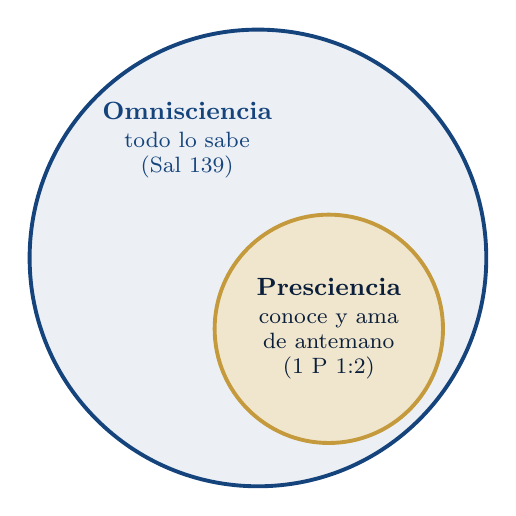
\begin{tikzpicture}
 \draw[azul,line width=1.4pt,fill=azul!8] (0,0) circle (2.9);
 \draw[dorado,line width=1.4pt,fill=dorado!25] (0.9,-0.9) circle (1.45);
 \node[font=\small\bfseries,text=azul,align=center] at (-0.9,1.5) {Omnisciencia\\[-1pt]\footnotesize\mdseries todo lo sabe\\[-2pt]\footnotesize\mdseries (Sal 139)};
 \node[font=\small\bfseries,text=azuloscuro,align=center] at (0.9,-0.9) {Presciencia\\[-1pt]\footnotesize\mdseries conoce y ama\\[-2pt]\footnotesize\mdseries de antemano\\[-2pt]\footnotesize\mdseries (1 P 1:2)};
\end{tikzpicture}\par
{\footnotesize\color{gris}\textit{Figura 1.} La presciencia como particularidad de la omnisciencia. \textit{Nota.} Elaboración propia.}
\end{center}

El verso que une esta obra invita a conocer a Dios: ``Mas alábese en esto el que se hubiere de alabar: en entenderme y conocerme, que yo soy \SENOR'' (Jer 9:24 [9:23]). El hebreo dice \heb{הַשְׂכֵּל וְיָדֹעַ אוֹתִי}, ``entender y conocerme''. Pablo corrige con delicadeza el orden de ese conocimiento: ``mas ahora, conociendo a Dios, o más bien, siendo conocidos por Dios'' (Gá 4:9). Antes de que nosotros lo conozcamos, él nos conoció. Este capítulo recorre ese orden.

En la clasificación de la serie, la omnisciencia es un atributo de \destacar{identidad}: responde a la pregunta ``¿quién es Dios?'', junto a la eternidad, la soberanía, la omnipotencia y la omnipresencia. Es \destacar{incomunicable}: el ser humano conoce ``en parte'' (1 Co 13:12) y recibe de Dios solo reflejos de su saber.

%===================================================================
\section{Texto ancla: el Salmo 139}

\subsection{``Tú me has examinado y conocido''}
La RVR1960 titula este salmo ``Omnipresencia y omnisciencia de Dios''. Es la confesión más personal de la Escritura sobre el conocimiento de Dios: David no habla de lo que Dios sabe del universo, sino de lo que sabe de él.

\hebverso{יְהוָה חֲקַרְתַּנִי וַתֵּדָע׃ אַתָּה יָדַעְתָּ שִׁבְתִּי וְקוּמִי בַּנְתָּה לְרֵעִי מֵרָחוֹק׃ \\ אָרְחִי וְרִבְעִי זֵרִיתָ וְכָל־דְּרָכַי הִסְכַּנְתָּה׃ כִּי אֵין מִלָּה בִּלְשׁוֹנִי הֵן יְהוָה יָדַעְתָּ כֻלָּהּ}
\begin{cita}Oh \SENOR{}, tú me has examinado y conocido. Tú has conocido mi sentarme y mi levantarme; Has entendido desde lejos mis pensamientos. Has escudriñado mi andar y mi reposo, Y todos mis caminos te son conocidos. Pues aún no está la palabra en mi lengua, Y he aquí, oh \SENOR{}, tú la sabes toda. Detrás y delante me rodeaste, Y sobre mí pusiste tu mano. Tal conocimiento es demasiado maravilloso para mí; Alto es, no lo puedo comprender.\fuente{(Sal 139:1--6)}\end{cita}

\begin{filologia}[Sal 139:1--4]
\begin{tabular}{@{}L{3.2cm}L{1.6cm}L{10cm}@{}}
\heb{חֲקַרְתַּנִי} \emph{jaqartani} & \heb{חקר} & ``me has examinado'': explorar a fondo, como los espías exploran una tierra (Jue 18:2) o el minero examina la roca (Job 28:3). \\[2pt]
\heb{וַתֵּדָע} \emph{vatedá} & \heb{ידע} & ``y (me) conociste'': el resultado del examen. El verbo se repite en los vv. 2, 4, 14 y dos veces en el v. 23. \\[2pt]
\heb{בַּנְתָּה} \emph{bantá} & \heb{בין} & ``has entendido'': discernir, distinguir una cosa de otra. \\[2pt]
\heb{לְרֵעִי} \emph{lerei} & \heb{רעה} & ``mis pensamientos'': palabra rara, solo aquí y en 139:17, de origen arameo según HALOT. \\[2pt]
\heb{זֵרִיתָ} \emph{zerita} & \heb{זרה} & ``has escudriñado'': el verbo de aventar el grano (Rt 3:2). Dios separa el trigo y la paja en el andar y el reposo. \\[2pt]
\heb{הִסְכַּנְתָּה} \emph{hiskanta} & \heb{סכן} & ``te son conocidos'': ser familiar, estar acostumbrado a algo. \\[2pt]
\heb{מִלָּה} \emph{milá} & \heb{מלל} & ``la palabra'' que todavía no llegó a la lengua (v. 4): Dios la conoce entera (\heb{כֻלָּהּ}). \\
\end{tabular}
\end{filologia}

\begin{nota}[Precisión]
Los significados siguen a HALOT (Koehler y Baumgartner, 2001). El matiz de ``aventar'' para \emph{zará} en el v. 3 lo proponen varios intérpretes por el uso del verbo en Rut 3:2; otros entienden ``medir'' o ``rodear''.
\end{nota}

Los verbos son concretos: sentarse, levantarse, andar, acostarse, hablar. El conocimiento de Dios no flota sobre la vida humana; entra en sus detalles ordinarios. Y el salmista no reacciona con una teoría, sino con asombro: ``Tal conocimiento es demasiado maravilloso para mí'' (\heb{פְּלִאיָה דַעַת מִמֶּנִּי}).

\subsection{Cuatro estrofas}
El salmo se suele dividir en cuatro estrofas de seis versos, aproximadamente:

\begin{center}\small\renewcommand{\arraystretch}{1.25}
\begin{tabular}{@{}L{2.0cm}L{3.0cm}L{9.4cm}@{}}
\toprule
\textbf{Versos} & \textbf{Tema} & \textbf{Contenido} \\ \midrule
1--6 & Me conoces & sentarse, levantarse, andar, hablar: nada se le escapa a Dios. \\
7--12 & Estás allí & cielo, Seol, alba, extremo del mar, tinieblas: no hay a dónde huir. \\
13--18 & Me formaste & el vientre, el embrión, el libro donde estaban escritos los días. \\
19--24 & Examíname & lo que el salmista confesó al comienzo, ahora lo pide. \\
\bottomrule
\end{tabular}\par
{\footnotesize\color{gris}\textit{Tabla 1.} Estructura del Salmo 139. \textit{Nota.} Elaboración propia.}
\end{center}

El salmo empieza y termina con los mismos dos verbos, \emph{jaqar} (``examinar'') y \emph{yadá} (``conocer''). En el v. 1 David \emph{confiesa}: ``tú me has examinado y conocido'' (\heb{חֲקַרְתַּנִי וַתֵּדָע}). En el v. 23 lo \emph{pide}: ``Examíname, oh Dios, y conoce mi corazón'' (\heb{חָקְרֵנִי אֵל וְדַע לְבָבִי}). Esa inclusión le da al salmo su movimiento: la omnisciencia pasa de ser una doctrina a ser una oración.

\begin{nota}[Precisión]
La división en cuatro estrofas es la usual en los comentarios; la inclusión entre los vv. 1 y 23 es una observación de la composición del salmo.
\end{nota}

La segunda estrofa (vv. 7--12) habla de la presencia de Dios más que de su conocimiento, y será objeto del estudio de la omnipresencia. Aquí basta notar que ambas perfecciones van juntas: Dios conoce todo porque está en todo lugar, y está en todo lugar sin dejar de conocerlo todo. ``Aun las tinieblas no encubren de ti, y la noche resplandece como el día'' (139:12).

\subsection{Antes de nacer: ``en tu libro''}
La tercera estrofa lleva el conocimiento de Dios hasta antes del nacimiento:

\hebverso{גָּלְמִי רָאוּ עֵינֶיךָ וְעַל־סִפְרְךָ כֻּלָּם יִכָּתֵבוּ \\ יָמִים יֻצָּרוּ וְלֹא אֶחָד בָּהֶם}
\begin{cita}No fue encubierto de ti mi cuerpo, Bien que en oculto fui formado, Y entretejido en lo más profundo de la tierra. Mi embrión vieron tus ojos, Y en tu libro estaban escritas todas aquellas cosas Que fueron luego formadas, Sin faltar una de ellas.\fuente{(Sal 139:15--16)}\end{cita}

\begin{filologia}[Sal 139:16]
\begin{tabular}{@{}L{3.2cm}L{1.6cm}L{10cm}@{}}
\heb{גָּלְמִי} \emph{golmí} & \heb{גלם} & ``mi embrión'': una masa todavía sin forma. Es la única aparición de la palabra en la Biblia. \\[2pt]
\heb{סִפְרְךָ} \emph{sifrejá} & \heb{ספר} & ``tu libro'': el registro de Dios (cf. Sal 56:8; Mal 3:16). \\[2pt]
\heb{יָמִים יֻצָּרוּ} \emph{yamim yutsaru} & \heb{יצר} & ``días que fueron formados'': el verbo del alfarero que formó al hombre del polvo (Gn 2:7). Dios ``formó'' los días como formó el cuerpo. \\
\end{tabular}
\end{filologia}

\begin{nota}[Precisión textual]
El final del v. 16 es difícil: la expresión \heb{וְלֹא אֶחָד בָּהֶם} admite dos lecturas según el texto escrito (\emph{ketiv}) y el leído (\emph{qeré}), y ``todas aquellas cosas'' puede referirse a los miembros del cuerpo o a los días de la vida. La RVR1960 lee lo primero; muchas versiones modernas leen ``los días que me fueron dados''. En ambos casos, el sentido central se mantiene: Dios conoció y dispuso la vida del salmista antes de que esta comenzara.
\end{nota}

Aquí la omnisciencia ya toma la forma de la presciencia. Dios vio a David antes de que tuviera forma, y escribió sus días antes de que llegara el primero. Lo mismo dirá el \SENOR{} a Jeremías: ``Antes que te formase en el vientre te conocí, y antes que nacieses te santifiqué'' (Jer 1:5). En ambos textos, el conocimiento previo no es una observación neutral: es cuidado, propósito y llamado.

\subsection{``Examíname, oh Dios''}

\hebverso{חָקְרֵנִי אֵל וְדַע לְבָבִי בְּחָנֵנִי וְדַע שַׂרְעַפָּי}
\begin{cita}Examíname, oh Dios, y conoce mi corazón; Pruébame y conoce mis pensamientos; Y ve si hay en mí camino de perversidad, Y guíame en el camino eterno.\fuente{(Sal 139:23--24)}\end{cita}

\begin{filologia}[Sal 139:23]
\begin{tabular}{@{}L{3.2cm}L{1.6cm}L{10cm}@{}}
\heb{חָקְרֵנִי} \emph{jaqreni} & \heb{חקר} & ``examíname'': el mismo verbo del v. 1, ahora en imperativo. \\[2pt]
\heb{בְּחָנֵנִי} \emph{bejaneni} & \heb{בחן} & ``pruébame'': probar como se prueba el metal en el fuego (Zac 13:9). \\[2pt]
\heb{שַׂרְעַפָּי} \emph{sarapái} & \heb{שׂרעף} & ``mis pensamientos'' inquietos o divididos (cf. Sal 94:19: ``la multitud de mis pensamientos''). \\
\end{tabular}
\end{filologia}

El que sabe que es conocido entero no tiene dónde esconderse, y por eso deja de intentarlo: se expone. El temor que podía producir la omnisciencia (``¿a dónde huiré?'', v. 7) termina convertido en confianza: ``guíame en el camino eterno''.

\begin{nota}[Precisión]
El gran rollo de los Salmos de la cueva 11 de Qumrán (11QPs\textsuperscript{a}, 11Q5) incluye el Salmo 139 dentro de su colección (Sanders, 1965). La columna y los versos conservados conviene verificarlos en la Leon Levy Dead Sea Scrolls Digital Library.
\end{nota}

%===================================================================
\section{Los Salmos: el Dios que ve, escudriña y cuenta}

El Salmo 139 no está solo. El salterio es el libro de Israel que más habla del conocimiento de Dios, y lo hace casi siempre en segunda persona: no describe lo que Dios sabe, sino que se lo dice a él en oración. ``Tú conoces'', ``tú has probado'', ``tú has contado''. En los Salmos, la omnisciencia no es un tema de discusión, sino el suelo sobre el que se ora. Esta sección recorre los salmos principales en el orden en que aparecen en el libro, desde el primero hasta el que alaba al Dios que cuenta las estrellas, y muestra cómo se sostienen entre sí. La tabla los reúne antes de exponerlos:

\begin{center}\small\renewcommand{\arraystretch}{1.18}
\begin{tabular}{@{}L{2.3cm}L{6.4cm}L{5.7cm}@{}}
\toprule
\textbf{Salmo} & \textbf{RVR1960} & \textbf{Qué conoce Dios} \\ \midrule
1:6 & ``\SENOR{} conoce el camino de los justos'' & el camino: conocer es cuidar \\
7:9 [7:10] & ``el Dios justo prueba la mente y el corazón'' & lo interior, para juzgar con justicia \\
11:4 & ``Sus ojos ven, sus párpados examinan'' & a los hijos de los hombres \\
17:3 & ``Tú has probado mi corazón, me has visitado de noche'' & lo que el justo es a solas \\
33:13--15 & ``Atento está a todas sus obras'' & a todos los moradores de la tierra \\
33:11 & ``El consejo de \SENOR{} permanecerá para siempre'' & su propio propósito, que no cambia \\
44:21 [44:22] & ``él conoce los secretos del corazón'' & lo escondido \\
56:8 [56:9] & ``Pon mis lágrimas en tu redoma'' & las huidas y las lágrimas \\
69:5 [69:6] & ``Dios, tú conoces mi insensatez'' & el pecado propio \\
90:8 & ``Nuestros yerros a la luz de tu rostro'' & el pecado oculto \\
94:9--11 & ``El que formó el ojo, ¿No verá?'' & los pensamientos del hombre \\
103:14 & ``él conoce nuestra condición'' & nuestra fragilidad \\
105:17 & ``Envió un varón delante de ellos'' & el futuro de su pueblo \\
113:5--6 & ``Que se humilla a mirar en el cielo y en la tierra'' & al pobre y a la estéril \\
139:1--24 & ``tú me has examinado y conocido'' & todo: actos, palabras, días \\
147:4--5 & ``su entendimiento es infinito'' & las estrellas, una por una \\
\bottomrule
\end{tabular}\par
{\footnotesize\color{gris}\textit{Tabla 2.} El conocimiento de Dios en los Salmos. \textit{Nota.} Elaboración propia; numeración española [hebrea] donde difiere.}
\end{center}

\subsection{Los dos caminos: el Salmo 1}
El salterio se abre con una afirmación sobre el conocimiento de Dios, y esa afirmación da el tono a todo el libro:

\hebverso{כִּי־יוֹדֵעַ יְהוָה דֶּרֶךְ צַדִּיקִים וְדֶרֶךְ רְשָׁעִים תֹּאבֵד}
\begin{cita}Porque \SENOR{} conoce el camino de los justos; Mas la senda de los malos perecerá.\fuente{(Sal 1:6)}\end{cita}

La frase no dice que Dios conozca el camino de los justos y desconozca el de los malos; Dios conoce los dos. Pero el paralelismo hebreo muestra que ``conocer'' aquí es más que saber: al camino conocido se opone el camino que ``perecerá''. Conocer el camino es guardarlo, sostenerlo y llevarlo a su término. Es el mismo sentido relacional de \emph{yadá} que se verá en Génesis 18:19 y Amós 3:2, y es la puerta por la que el salterio entra en el tema: el Dios que todo lo sabe conoce de un modo particular a los suyos. Desde el primer salmo, la omnisciencia ya contiene el germen de la presciencia.

\subsection{Sus ojos ven, sus párpados examinan: los Salmos 7, 11 y 17}
Tres salmos de David, escritos en momentos de acusación y persecución, apelan al Dios que examina. El primero lo hace en medio de una calumnia:

\hebverso{וּבֹחֵן לִבּוֹת וּכְלָיוֹת אֱלֹהִים צַדִּיק}
\begin{cita}Fenezca ahora la maldad de los inicuos, mas establece tú al justo; Porque el Dios justo prueba la mente y el corazón.\fuente{(Sal 7:9 [7:10])}\end{cita}

El segundo responde a quienes aconsejan huir al monte como un ave, porque los fundamentos se han destruido (11:1--3). David no huye, porque el trono de Dios no se ha movido:

\hebverso{יְהוָה בַּשָּׁמַיִם כִּסְאוֹ עֵינָיו יֶחֱזוּ עַפְעַפָּיו יִבְחֲנוּ בְּנֵי אָדָם}
\begin{cita}\SENOR{} está en su santo templo; \SENOR{} tiene en el cielo su trono; Sus ojos ven, sus párpados examinan a los hijos de los hombres. \SENOR{} prueba al justo; Pero al malo y al que ama la violencia, su alma los aborrece.\fuente{(Sal 11:4--5)}\end{cita}

El tercero es la oración de un justo que se deja examinar de noche:

\hebverso{בָּחַנְתָּ לִבִּי פָּקַדְתָּ לַּיְלָה צְרַפְתַּנִי בַל־תִּמְצָא}
\begin{cita}Tú has probado mi corazón, me has visitado de noche; Me has puesto a prueba, y nada inicuo hallaste; He resuelto que mi boca no haga transgresión.\fuente{(Sal 17:3)}\end{cita}

\begin{filologia}[Sal 7:9; 11:4; 17:3]
\begin{tabular}{@{}L{3.2cm}L{1.6cm}L{10cm}@{}}
\heb{בֹּחֵן} \emph{bojén} & \heb{בחן} & ``el que prueba'': participio, una acción constante. Es el verbo del ensayo de los metales, el mismo de Sal 139:23 (``pruébame'') y Jer 17:10. \\[2pt]
\heb{לִבּוֹת וּכְלָיוֹת} \emph{libot uj\-layot} & \heb{לב}; \heb{כליה} & ``corazones y riñones'' (RVR1960: ``la mente y el corazón''). En la antropología hebrea los riñones son la sede de lo más íntimo: emociones y deseos que nadie ve. \\[2pt]
\heb{יֶחֱזוּ} \emph{yejezú} & \heb{חזה} & ``ven'', ``contemplan'': el verbo de la visión atenta, del que viene \emph{jazón}, ``visión'' profética. \\[2pt]
\heb{עַפְעַפָּיו} \emph{afapav} & \heb{עפעף} & ``sus párpados'': una imagen humana para el examen detenido, como quien entrecierra los ojos para mirar mejor. \\[2pt]
\heb{פָּקַדְתָּ} \emph{pacadta} & \heb{פקד} & ``visitaste'', ``inspeccionaste'': la visita de Dios para revisar y cuidar. \\[2pt]
\heb{צְרַפְתַּנִי} \emph{tseraftani} & \heb{צרף} & ``me refinaste'', como el orfebre que funde la plata (Sal 12:6; 66:10). \\
\end{tabular}
\end{filologia}

\begin{nota}[Precisión]
La lectura de los ``párpados'' como imagen del examen detenido es una explicación usual de los comentarios; el texto solo pone en paralelo ``sus ojos ven'' y ``sus párpados examinan''.
\end{nota}

Los tres salmos comparten un movimiento. El justo acusado no busca otro tribunal; apela al Dios que ve lo que los acusadores no ven. El examen divino, que podría producir miedo, se vuelve refugio para el inocente y advertencia para el violento. Y el examen no se hace desde lejos: los ojos que están ``en el cielo'' (11:4) son los que visitan ``de noche'' (17:3). El trono y la alcoba no están separados para el Dios que conoce.

\subsection{Desde su morada miró: el Salmo 33}

\hebverso{מִמְּכוֹן־שִׁבְתּוֹ הִשְׁגִּיחַ אֶל כָּל־יֹשְׁבֵי הָאָרֶץ \\ הַיֹּצֵר יַחַד לִבָּם הַמֵּבִין אֶל־כָּל־מַעֲשֵׂיהֶם}
\begin{cita}Desde los cielos miró \SENOR{}; Vio a todos los hijos de los hombres; Desde el lugar de su morada miró Sobre todos los moradores de la tierra. El formó el corazón de todos ellos; Atento está a todas sus obras.\fuente{(Sal 33:13--15)}\end{cita}

\begin{filologia}[Sal 33:14--15]
\begin{tabular}{@{}L{3.2cm}L{1.6cm}L{10cm}@{}}
\heb{הִשְׁגִּיחַ} \emph{hishguíaj} & \heb{שׁגח} & ``miró'' con atención. La raíz aparece solo tres veces en la Biblia (Sal 33:14; Cnt 2:9; Is 14:16). De ella el hebreo posterior formó \emph{hashgajá}, la palabra judía para ``providencia''. \\[2pt]
\heb{הַיֹּצֵר יַחַד לִבָּם} & \heb{יצר} & ``el que formó el corazón de todos ellos'': el que hizo el corazón lo conoce. \\[2pt]
\heb{הַמֵּבִין} \emph{hamevín} & \heb{בין} & ``atento está'', el que entiende y discierne. \\
\end{tabular}
\end{filologia}

El argumento del salmo es el de un artesano: el que formó (\emph{yotser}, el verbo del alfarero de Gn 2:7) el corazón de cada hombre entiende cada obra que de ese corazón procede. Pero el mismo salmo, unos versos antes, pone otra cosa junto a esa mirada universal:

\hebverso{עֲצַת יְהוָה לְעוֹלָם תַּעֲמֹד מַחְשְׁבוֹת לִבּוֹ לְדֹר וָדֹר}
\begin{cita}\SENOR{} hace nulo el consejo de las naciones, Y frustra las maquinaciones de los pueblos. El consejo de \SENOR{} permanecerá para siempre; Los pensamientos de su corazón por todas las generaciones.\fuente{(Sal 33:10--11)}\end{cita}

Dios conoce los planes de las naciones y los anula; su propio consejo (\heb{עֲצַת יְהוָה}) permanece. El salmo junta así lo que Isaías dirá con más fuerza (``mi consejo permanecerá'', Is 46:10) y lo que Pedro predicará en Pentecostés: el saber de Dios sobre el futuro va unido a su propósito. Y el salmo termina con una mirada de favor: ``He aquí el ojo de \SENOR{} sobre los que le temen, Sobre los que esperan en su misericordia'' (33:18). El ojo que ve a todos descansa de un modo particular sobre los que esperan en él.

\subsection{Ningún secreto: los Salmos 44, 69 y 38}
En otros salmos, la omnisciencia aparece en la confesión. El Salmo 44 la usa como argumento de un pueblo que sufre sin haber abandonado a su Dios: ``Si nos hubiésemos olvidado del nombre de nuestro Dios, O alzado nuestras manos a dios ajeno, ¿No demandaría Dios esto? Porque él conoce los secretos del corazón'' (Sal 44:20--21 [44:21--22]). La palabra hebrea es \heb{תַּעֲלֻמוֹת לֵב} (\emph{taalumot lev}), ``las cosas escondidas del corazón'', de la raíz \heb{עלם}, ``ocultar''. El que escribe sabe que no podría engañar a Dios, y por eso apela a él.

El Salmo 69 hace la confesión opuesta, la del pecador: ``Dios, tú conoces mi insensatez, Y mis pecados no te son ocultos'' (Sal 69:5 [69:6]). Y el Salmo 38, en medio del dolor, convierte el mismo saber en descanso: ``Señor, delante de ti están todos mis deseos, Y mi suspiro no te es oculto'' (Sal 38:9 [38:10]). Es notable que este último verso no use el Nombre sino \heb{אֲדֹנָי} (\emph{Adonay}), ``Señor'': el que conoce el suspiro es el Señor soberano. Inocencia, culpa y dolor se dicen delante del mismo Dios, porque nada de eso le está escondido. Moisés, en el Salmo 90, lo resume como oración comunitaria: ``Pusiste nuestras maldades delante de ti, Nuestros yerros a la luz de tu rostro'' (90:8). Pink (2020, p. 16) llama a este verso ``solemne'', porque nadie puede rechazar a Dios sin estar ya a la luz de su rostro.

\subsection{El que formó el ojo: el Salmo 94}
El Salmo 94 responde a los que dicen que Dios no ve:

\hebverso{הֲנֹטַע אֹזֶן הֲלֹא יִשְׁמָע אִם־יֹצֵר עַיִן הֲלֹא יַבִּיט \\ הֲיֹסֵר גּוֹיִם הֲלֹא יוֹכִיחַ הַמְלַמֵּד אָדָם דָּעַת}
\begin{cita}Y dijeron: No verá JAH, Ni entenderá el Dios de Jacob. Entended, necios del pueblo; Y vosotros, fatuos, ¿cuándo seréis sabios? El que hizo el oído, ¿No oirá? El que formó el ojo, ¿No verá? El que castiga a las naciones, ¿No reprenderá? ¿No sabrá el que enseña al hombre la ciencia? \SENOR{} conoce los pensamientos de los hombres, Que son vanidad.\fuente{(Sal 94:7--11)}\end{cita}

El argumento va del Creador a su obra. Quien diseñó el oído no puede ser sordo; quien formó el ojo no puede ser ciego; quien ``enseña al hombre \emph{dáat}'' (conocimiento) no puede ignorar. Todo saber humano es prestado. ``No verá Jah'' es la teología del impío (cf. Sal 10:11), y el salmo la llama necedad. Unos versos después, el mismo salmo da la consecuencia para Israel: ``Porque no abandonará \SENOR{} a su pueblo, Ni desamparará su heredad'' (94:14). Pablo citará ese verso cuando hable de la presciencia de Dios sobre Israel (Ro 11:1--2).

\subsection{Conoce nuestra condición: el Salmo 103}

\hebverso{כְּרַחֵם אָב עַל־בָּנִים רִחַם יְהוָה עַל־יְרֵאָיו \\ כִּי־הוּא יָדַע יִצְרֵנוּ זָכוּר כִּי־עָפָר אֲנָחְנוּ}
\begin{cita}Como el padre se compadece de los hijos, Se compadece \SENOR{} de los que le temen. Porque él conoce nuestra condición; Se acuerda de que somos polvo.\fuente{(Sal 103:13--14)}\end{cita}

\begin{filologia}[Sal 103:14]
\begin{tabular}{@{}L{3.2cm}L{1.6cm}L{10cm}@{}}
\heb{יָדַע} \emph{yadá} & \heb{ידע} & ``conoce'': el verbo central del atributo. \\[2pt]
\heb{יִצְרֵנוּ} \emph{yitsrenu} & \heb{יצר} & ``nuestra condición'', literalmente ``nuestra hechura'', ``cómo estamos formados''. Es la raíz del alfarero que formó al hombre del polvo (Gn 2:7), la de Sal 33:15 (``el formó el corazón'') y la de Sal 139:16 (``días que fueron formados''). \\[2pt]
\heb{עָפָר} \emph{afar} & --- & ``polvo'': la materia de Gn 2:7 y de Gn 3:19, ``pues polvo eres''. \\
\end{tabular}
\end{filologia}

David une aquí dos verbos que en hebreo son vecinos: Dios ``conoce'' y Dios ``se acuerda''. El que conoce cómo nos formó no espera de nosotros lo que el polvo no puede dar. Su saber es el de un padre: no un registro de faltas, sino una compasión informada. Pink (2020, p. 16) toma este verso como consuelo para los tiempos de ``cansancio y debilidad''. El Salmo 103 muestra que la omnisciencia no compite con la misericordia, sino que la hace exacta: Dios se compadece porque sabe.

\begin{nota}[Precisión]
El Talmud lee los cinco ``Bendice, alma mía'' de los Salmos 103 y 104 como dichos del alma frente a Dios, y compara: así como el Santo, bendito sea, llena el mundo, el alma llena el cuerpo; así como él ve y no es visto, el alma ve y no es vista (\emph{Berajot} 10a). La omnisciencia aparece allí en la fórmula ``ve y no es visto''. Traducción y paráfrasis propias; conviene cotejar el texto en Sefaria.
\end{nota}

\subsection{Se humilla a mirar: el Salmo 113}
El Salmo 113 abre el \emph{Hallel}, los salmos de alabanza (113--118) que Israel cantaba en las fiestas. Su centro es una pregunta y una imagen del conocimiento de Dios:

\hebverso{מִי כַּיהוָה אֱלֹהֵינוּ הַמַּגְבִּיהִי לָשָׁבֶת \\ הַמַּשְׁפִּילִי לִרְאוֹת בַּשָּׁמַיִם וּבָאָרֶץ}
\begin{cita}Excelso sobre todas las naciones es \SENOR{}, Sobre los cielos su gloria. ¿Quién como \SENOR{} nuestro Dios, Que se sienta en las alturas, Que se humilla a mirar En el cielo y en la tierra? El levanta del polvo al pobre, Y al menesteroso alza del muladar, Para hacerlos sentar con los príncipes, Con los príncipes de su pueblo. El hace habitar en familia a la estéril, Que se goza en ser madre de hijos. Aleluya.\fuente{(Sal 113:4--9)}\end{cita}

\begin{filologia}[Sal 113:5--9]
\begin{tabular}{@{}L{3.2cm}L{1.6cm}L{10cm}@{}}
\heb{הַמַּגְבִּיהִי לָשָׁבֶת} & \heb{גבה} & ``el que se eleva para sentarse'': el trono más alto. \\[2pt]
\heb{הַמַּשְׁפִּילִי לִרְאוֹת} & \heb{שׁפל}; \heb{ראה} & ``el que se abaja para ver''. Los dos participios forman un contraste: el más alto es el que más se inclina. El verbo de ver es el de \emph{El roí} (Gn 16:13). \\[2pt]
\heb{מְקִימִי מֵעָפָר דָּל} & \heb{קום} & ``el que levanta del polvo al pobre'': casi palabra por palabra el cántico de Ana (1 S 2:8). \\[2pt]
\heb{עֲקֶרֶת הַבַּיִת} & \heb{עקר} & ``la estéril de la casa'', a la que Dios hace ``madre gozosa de hijos'' (\heb{אֵם־הַבָּנִים שְׂמֵחָה}). \\
\end{tabular}
\end{filologia}

El salmo pone la grandeza y la mirada de Dios en un mismo movimiento. El \SENOR{} está ``sobre los cielos'', pero no se queda allí: ``se humilla a mirar''. Su conocimiento no es el de un observador que mira de lejos, sino el de quien se inclina hasta el polvo y el muladar, y mira para actuar: levanta al pobre, sienta al menesteroso con los príncipes, da hijos a la estéril. Rashi observa que los participios de estos versos llevan una \emph{yod} que sobra en la gramática (\emph{magbihí}, \emph{mashpilí}, \emph{meqimí}, \emph{lehoshibí}, \emph{moshibí}), como si el poeta subrayara cada acción de Dios.

El salmo tiene, además, una deuda visible con el cántico de Ana. Su v. 7 repite el verso de 1 S 2:8: ``El levanta del polvo al pobre, Y del muladar exalta al menesteroso'' (\heb{מֵקִים מֵעָפָר דָּל מֵאַשְׁפֹּת יָרִים אֶבְיוֹן}), y su v. 9 canta lo que Ana vivió, la estéril hecha madre. El mismo cántico que llama al \SENOR{} \emph{El deot}, ``el Dios de todo saber'' (1 S 2:3), que se estudia enseguida, resuena en el salmo que dice que ese Dios ``se humilla a mirar''. Por eso el Salmo 113 completa al 139: el 139 confiesa que Dios lo sabe todo; el 113 muestra hacia dónde mira primero el que lo sabe todo.

\begin{nota}[Precisión]
La Misná discute hasta dónde se canta el \emph{Hallel} en la noche de Pascua: la escuela de Shamai dice ``hasta `madre gozosa de hijos' '' (Sal 113:9), y la de Hilel, ``hasta `el pedernal en fuente de aguas' '' (Sal 114:8) (\emph{Pesajim} 10:6). El Talmud enseña que ``en todo lugar donde encuentras la grandeza del Santo, bendito sea, allí encuentras su humildad'' (\emph{Meguilá} 31a), y lo prueba con Dt 10:17--18, Is 57:15 y Sal 68:4--5; la aplicación al Salmo 113 es propia. Rashi a Sal 113:5, según Sefaria. Que el ``himno'' de Mt 26:30 fuera el \emph{Hallel} es una lectura frecuente, no explícita en el texto.
\end{nota}

\subsection{Cuenta las estrellas y guarda las lágrimas: los Salmos 147 y 56}

\hebverso{מוֹנֶה מִסְפָּר לַכּוֹכָבִים לְכֻלָּם שֵׁמוֹת יִקְרָא \\ גָּדוֹל אֲדוֹנֵינוּ וְרַב־כֹּחַ לִתְבוּנָתוֹ אֵין מִסְפָּר}
\begin{cita}El sana a los quebrantados de corazón, Y venda sus heridas. El cuenta el número de las estrellas; A todas ellas llama por sus nombres. Grande es el Señor nuestro, y de mucho poder; Y su entendimiento es infinito.\fuente{(Sal 147:3--5)}\end{cita}

\begin{filologia}[Sal 147:4--5]
\begin{tabular}{@{}L{3.2cm}L{1.6cm}L{10cm}@{}}
\heb{מוֹנֶה מִסְפָּר} \emph{moné mispar} & \heb{מנה}; \heb{ספר} & ``el que cuenta el número'' de las estrellas. \\[2pt]
\heb{לְכֻלָּם שֵׁמוֹת יִקְרָא} & \heb{קרא} & ``a todas ellas llama por nombres'': conocer por nombre es conocer a cada una (cf. Is 40:26). \\[2pt]
\heb{לִתְבוּנָתוֹ אֵין מִסְפָּר} & \heb{בין} & ``de su entendimiento no hay número'' (RVR1960: ``es infinito''). \\
\end{tabular}
\end{filologia}

El juego de palabras es intencional: el que da ``número'' (\emph{mispar}) a las estrellas tiene un entendimiento ``sin número'' (\emph{ein mispar}). El que cuenta no puede ser contado. Pero el salmo no empieza por las estrellas, sino por las heridas: ``El sana a los quebrantados de corazón'' (147:3). El mismo conocimiento que nombra las estrellas venda las heridas de un corazón roto. Pink (2020, p. 17) parte de este verso para afirmar que el saber de Dios abarca el pasado, el presente y el futuro, ``desde el más mínimo hasta el mayor'' de los eventos. El verbo de contar aparece en otro salmo, en boca de un fugitivo:

\begin{cita}Mis huidas tú has contado; Pon mis lágrimas en tu redoma; ¿No están ellas en tu libro?\fuente{(Sal 56:8 [56:9])}\end{cita}

\begin{filologia}[Sal 56:8 (56:9 en hebreo)]
\begin{tabular}{@{}L{3.2cm}L{1.6cm}L{10cm}@{}}
\heb{נֹדִי סָפַרְתָּה} \emph{nodí safarta} & \heb{ספר} & ``mi andar errante lo contaste'': el verbo de contar, de la misma raíz que ``libro''. \\[2pt]
\heb{בְנֹאדֶךָ} \emph{venodeja} & \heb{נאד} & ``en tu odre'' (``redoma''). Juego de palabras con \heb{נֹד} (\emph{nod}), ``huida'': las huidas se guardan en el odre de Dios. \\[2pt]
\heb{בְּסִפְרָתֶךָ} \emph{besifrateja} & \heb{ספר} & ``en tu libro'', ``en tu registro''. \\
\end{tabular}
\end{filologia}

David escribió este salmo cuando los filisteos lo prendieron en Gat (título del salmo; cf. 1 S 21:10--15). Dios lleva la cuenta del universo y de las lágrimas de un hombre que huye. La grandeza y la ternura son el mismo conocimiento.

\subsection{El cántico de Ana: \emph{El deot}}\label{subsec:eldeot-omnis}
Fuera del salterio, pero en un poema, aparece el título más preciso que la Biblia hebrea da al Dios que todo lo sabe:

\hebverso{כִּי אֵל דֵּעוֹת יְהוָה וְלוֹ נִתְכְּנוּ עֲלִלוֹת}
\begin{cita}No multipliquéis palabras de grandeza y altanería; Cesen las palabras arrogantes de vuestra boca; Porque el Dios de todo saber es \SENOR{}, Y a él toca el pesar las acciones.\fuente{(1 S 2:3)}\end{cita}

\begin{filologia}[1 S 2:3]
\begin{tabular}{@{}L{3.2cm}L{1.6cm}L{10cm}@{}}
\heb{אֵל דֵּעוֹת} \emph{El deot} & \heb{ידע} & ``Dios de conocimientos'': el plural expresa plenitud. La LXX traduce \grc{θεὸς γνώσεων}. \\[2pt]
\heb{נִתְכְּנוּ} \emph{nitkenu} & \heb{תכן} & ``son pesadas'', medidas en la balanza. Dios no solo conoce las acciones: las evalúa. \\
\end{tabular}
\end{filologia}

\begin{nota}[Precisión textual]
El texto escrito (\emph{ketiv}) dice \heb{וְלֹא}, ``y no (son pesadas)''; el texto leído (\emph{qeré}) dice \heb{וְלוֹ}, ``y por él (son pesadas)''. La RVR1960 sigue el \emph{qeré}: ``y a él toca el pesar las acciones''.
\end{nota}

Ana, una mujer estéril humillada por su rival, canta que el \SENOR{} es \emph{El deot}. El conocimiento de Dios aparece aquí como consuelo del humilde y advertencia al arrogante: Dios conoce lo que pasó en Silo, y pesa las palabras altivas. Este título será retomado en Qumrán, como se verá más adelante.

\subsection{Los Salmos que miran hacia adelante}
El salterio también confiesa que Dios conoce de antemano. El Salmo 139 lo dice de una vida: ``en tu libro estaban escritas todas aquellas cosas'' (139:16). El Salmo 105 lo dice de la historia de Israel, al recordar a José:

\hebverso{שָׁלַח לִפְנֵיהֶם אִישׁ לְעֶבֶד נִמְכַּר יוֹסֵף}
\begin{cita}Trajo hambre sobre la tierra, Y quebrantó todo sustento de pan. Envió un varón delante de ellos; A José, que fue vendido por siervo. Afligieron sus pies con grillos; En cárcel fue puesta su persona. Hasta la hora que se cumplió su palabra, El dicho de \SENOR{} le probó.\fuente{(Sal 105:16--19)}\end{cita}

Lo que los hermanos de José hicieron por envidia, Dios lo había visto antes del hambre, y envió ``delante'' al que los salvaría. Es lo que José mismo dijo a sus hermanos: ``Vosotros pensasteis mal contra mí, mas Dios lo encaminó a bien'' (Gn 50:20). El salmo une, como lo hará Pedro, el pecado de los hombres y el propósito previo de Dios.

Y hay salmos que la fe de Israel y la de los apóstoles leyeron como palabra dicha de antemano sobre el Mesías: el Salmo 2 (``Mi hijo eres tú''), el 16 (``no dejarás mi alma en el Seol''), el 110 (``Siéntate a mi diestra'') y el 118 (``La piedra que desecharon los edificadores''). El Nuevo Testamento los cita como prueba de que Dios sabía y había dicho lo que haría en Cristo: ``era necesario que se cumpliese todo lo que está escrito de mí en la ley de Moisés, en los profetas y en los salmos'' (Lc 24:44). Pink (2020, p. 18) ve en estas profecías cumplidas la ilustración más clara del conocimiento perfecto de Dios. Pedro será el apóstol que más los use, como se verá en la sección dedicada a Cristo.

\begin{center}
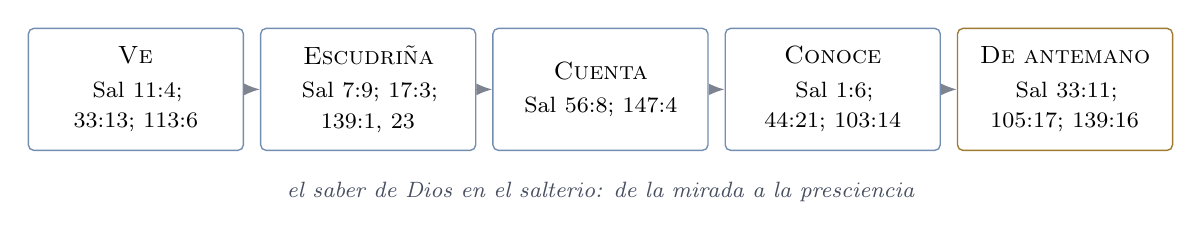
\begin{tikzpicture}[font=\small]
 \tikzset{caja/.style={draw=azul!60,line width=0.5pt,fill=white,rounded corners=2pt,text width=2.45cm,align=center,inner sep=4pt,minimum height=1.55cm}}
 \node[caja] (a) at (0,0) {\textsc{Ve}\\[1pt]{\footnotesize Sal 11:4; 33:13; 113:6}};
 \node[caja] (b) at (2.95,0) {\textsc{Escudriña}\\[1pt]{\footnotesize Sal 7:9; 17:3; 139:1, 23}};
 \node[caja] (c) at (5.9,0) {\textsc{Cuenta}\\[1pt]{\footnotesize Sal 56:8; 147:4}};
 \node[caja] (d) at (8.85,0) {\textsc{Conoce}\\[1pt]{\footnotesize Sal 1:6; 44:21; 103:14}};
 \node[caja,draw=dorado!80!black] (e) at (11.8,0) {\textsc{De antemano}\\[1pt]{\footnotesize Sal 33:11; 105:17; 139:16}};
 \foreach \p/\q in {a/b,b/c,c/d,d/e}{\draw[gris!70,line width=0.5pt,-{Latex[length=2mm]}] (\p) -- (\q);}
 \node[font=\footnotesize\itshape,text=gris] at (5.9,-1.3) {el saber de Dios en el salterio: de la mirada a la presciencia};
\end{tikzpicture}\par
{\footnotesize\color{gris}\textit{Figura 2.} Lo que los Salmos confiesan del conocimiento de Dios. \textit{Nota.} Elaboración propia.}
\end{center}

%===================================================================
\section{La palabra: conocer de cerca}

\subsection{\emph{Yadá} en lo concreto}
El hebreo no tiene una palabra técnica para ``omnisciencia''. La expresa con verbos concretos, y el principal es \heb{יָדַע} (\emph{yadá}), ``conocer, saber''. La raíz aparece unas 940 veces en el Antiguo Testamento, y su uso muestra que no se limita a tener información:

\begin{center}\small\renewcommand{\arraystretch}{1.2}
\begin{tabular}{@{}L{2.0cm}L{6.4cm}L{6.0cm}@{}}
\toprule
\textbf{Texto} & \textbf{Uso de \heb{ידע}} & \textbf{Matiz} \\ \midrule
Gn 4:1 & ``Conoció Adán a su mujer Eva'' & intimidad conyugal \\
Gn 18:19 & ``Porque yo sé'' (\heb{יְדַעְתִּיו}, ``lo he conocido'') & elección con propósito \\
Éx 2:25 & ``y los reconoció Dios'' (\heb{וַיֵּדַע}) & compasión ante el sufrimiento \\
Éx 33:17 & ``te he conocido por tu nombre'' & favor personal \\
Jer 1:5 & ``Antes que te formase en el vientre te conocí'' & conocimiento previo y llamado \\
Am 3:2 & ``A vosotros solamente he conocido'' & elección del pacto \\
Os 13:5 & ``Yo te conocí en el desierto'' & cuidado en la prueba \\
Sal 1:6 & ``\SENOR{} conoce el camino de los justos'' & aprobación y protección \\
\bottomrule
\end{tabular}\par
{\footnotesize\color{gris}\textit{Tabla 3.} Usos de \emph{yadá} con matiz relacional. \textit{Nota.} Elaboración propia.}
\end{center}

Amós 3:2 es el texto decisivo: ``A vosotros solamente he conocido de todas las familias de la tierra''. No puede significar ``solo de vosotros tengo información'', porque el mismo libro dice que Dios conoce a todas las naciones (Am 9:7). Significa ``solo a vosotros escogí''. Cuando Dios es el sujeto, \emph{yadá} con frecuencia significa conocer con favor, escoger, amar.

\begin{nota}[Precisión]
El conteo es propio, con la RVR1960 etiquetada con números Strong (H3045: 938 apariciones en 872 versículos); conviene verificarlo en e-Sword. El sentido de cada uso lo fija su contexto y no la etimología: Carson (2013) advierte contra la ``falacia de la raíz'', que proyecta sobre cada texto el supuesto sentido original de una palabra. Aquí el argumento no es que \emph{yadá} ``siempre'' signifique amar, sino que en ciertos contextos, con Dios como sujeto, lo significa.
\end{nota}

\subsection{``Yo lo he conocido'': Génesis 18:19}

\hebverso{כִּי יְדַעְתִּיו לְמַעַן אֲשֶׁר יְצַוֶּה אֶת־בָּנָיו וְאֶת־בֵּיתוֹ אַחֲרָיו}
\begin{cita}Porque yo sé que mandará a sus hijos y a su casa después de sí, que guarden el camino de \SENOR{}, haciendo justicia y juicio, para que haga venir \SENOR{} sobre Abraham lo que ha hablado acerca de él.\fuente{(Gn 18:19)}\end{cita}

\begin{filologia}[Gn 18:19]
\begin{tabular}{@{}L{3.2cm}L{1.6cm}L{10cm}@{}}
\heb{יְדַעְתִּיו} \emph{yedativ} & \heb{ידע} & ``lo he conocido'': perfecto con sufijo de objeto (``a él''), no ``sé que''. \\[2pt]
\heb{לְמַעַן אֲשֶׁר} \emph{lemaan asher} & --- & ``para que'': indica propósito. La obediencia de Abraham es el fruto, no la causa, del conocimiento de Dios. \\
\end{tabular}
\end{filologia}

La RVR1960 traduce ``yo sé que mandará'', siguiendo la lectura que también tiene el Targum. Rashi discute esa lectura: si se entendiera ``sé que mandará'', la expresión ``para que'' no encajaría en la frase. Por eso explica \emph{yedativ} como \emph{leshón jibá}, ``expresión de cariño'', ``porque el que ama a una persona la acerca, la conoce y la reconoce''.

\begin{nota}[Precisión]
Rashi a Gn 18:19, según Sefaria; la traducción del comentario es propia. Rashi compara este uso con \emph{modá} (``pariente'') en Rut 2:1.
\end{nota}

\subsection{La familia del conocer}
Junto a \emph{yadá}, el hebreo usa otros verbos para el conocimiento de Dios. Cada uno añade un matiz: Dios \emph{ve}, \emph{escudriña}, \emph{prueba}, \emph{discierne}, \emph{vigila}.

\begin{center}\small\renewcommand{\arraystretch}{1.2}
\begin{tabular}{@{}L{3.2cm}L{1.1cm}L{6.0cm}L{4.1cm}@{}}
\toprule
\textbf{Término} & \textbf{Veces} & \textbf{Sentido y RVR1960} & \textbf{Textos} \\ \midrule
\heb{יָדַע} \emph{yadá} & 938 & conocer, saber; ``reconocer'' & Gn 18:19; Sal 139:1 \\
\heb{דַּעַת} \emph{dáat} & 93 & conocimiento; ``ciencia'', ``sabiduría'' & Sal 94:10; 139:6 \\
\heb{דֵּעָה} \emph{deá} & 6 & saber; ``Dios de todo saber'' & 1 S 2:3; Is 11:9 \\
\heb{תְּמִים דֵּעִים} & 1 & ``el Perfecto en sabiduría'' & Job 37:16 \\
\heb{חָקַר} \emph{jaqar} & 26 & examinar, escudriñar & Sal 139:1, 23; Jer 17:10 \\
\heb{בָּחַן} \emph{bajan} & 29 & probar (como al metal) & Sal 7:9 [7:10]; 139:23 \\
\heb{בִּין}; \heb{תְּבוּנָה} & 168; 42 & entender; entendimiento & Sal 139:2; 147:5 \\
\heb{רָאָה} \emph{raá} & --- & ver; ``proveer'' (Gn 22:8, 14) & Gn 16:13; Éx 3:7 \\
\heb{שָׁגַח} \emph{shagaj} & 3 & mirar con atención & Sal 33:14 \\
\heb{צָפָה} \emph{tsafá} & 35 & vigilar; ``mirando'' & Pr 15:3 \\
\bottomrule
\end{tabular}\par
{\footnotesize\color{gris}\textit{Tabla 4.} Espectro hebreo del conocimiento de Dios. \textit{Nota.} Conteos propios con la RVR1960-Strong (H3045, H1847, H2713, H974, H995, H8394, H7688, H6822); \emph{deá} según los léxicos (1 S 2:3; Job 36:4; Sal 73:11; Is 11:9; 28:9; Jer 3:15). \emph{Raá} se usa más de mil veces y no se cuenta. Verificar en e-Sword.}
\end{center}

Dos expresiones merecen atención. \heb{תְּמִים דֵּעִים} (\emph{temim deím}, Job 37:16), ``perfecto en conocimientos'', es lo más cercano a un término técnico para la omnisciencia en la Biblia hebrea. Y \heb{אֵל רֳאִי} (\emph{El roí}, Gn 16:13), ``Dios que me ve'', es el nombre que le da Agar, una esclava egipcia, en el desierto: un nombre de Dios que nace de haber sido vista por él, y que se estudia en la sección~\ref{sec:nombre-omnis}.

\subsection{El espectro griego}

\begin{center}\small\renewcommand{\arraystretch}{1.2}
\begin{tabular}{@{}L{3.0cm}L{1.0cm}L{4.4cm}L{6.0cm}@{}}
\toprule
\textbf{Término} & \textbf{NA27} & \textbf{Sentido} & \textbf{Textos} \\ \midrule
\grc{γινώσκω} & 222 & conocer & 1 Co 8:3; Gá 4:9; 2 Ti 2:19 \\
\grc{γνῶσις} & 29 & conocimiento & Ro 11:33; Col 2:3 \\
\grc{προγινώσκω} & 5 & conocer de antemano & Hch 26:5; Ro 8:29; 11:2; 1 P 1:20; 2 P 3:17 \\
\grc{πρόγνωσις} & 2 & presciencia & Hch 2:23; 1 P 1:2 \\
\grc{καρδιογνώστης} & 2 & ``conocedor de corazones'' & Hch 1:24; 15:8 \\
\grc{ἐραυνάω} & 6 & escudriñar & Ro 8:27; 1 Co 2:10; Ap 2:23 \\
\grc{ἀνεξεραύνητος} & 1 & insondable & Ro 11:33 \\
\grc{ἀνεξιχνίαστος} & 2 & sin huella, inescrutable & Ro 11:33; Ef 3:8 \\
\bottomrule
\end{tabular}\par
{\footnotesize\color{gris}\textit{Tabla 5.} Espectro griego. \textit{Nota.} Conteo propio con el NA27 etiquetado con números Strong (G1097, G1108, G4267, G4268, G2589, G2045, G419, G421).}
\end{center}

\subsection{``Presciencia'' en la RVR1960}
La palabra ``presciencia'' aparece una sola vez en la RVR1960 (1 P 1:2). Las otras apariciones del grupo \grc{πρόγνωσις}/\grc{προγινώσκω} se traducen con paráfrasis:

\begin{center}\small\renewcommand{\arraystretch}{1.2}
\begin{tabular}{@{}L{1.7cm}L{3.1cm}L{4.9cm}L{4.7cm}@{}}
\toprule
\textbf{Texto} & \textbf{Griego} & \textbf{RVR1960} & \textbf{Objeto} \\ \midrule
Hch 2:23 & \grc{προγνώσει} & ``anticipado conocimiento'' & Jesús (``a éste'') \\
Hch 26:5 & \grc{προγινώσκοντες} & ``saben\ldots{} desde el principio'' & los judíos conocían a Pablo \\
Ro 8:29 & \grc{προέγνω} & ``a los que antes conoció'' & los creyentes \\
Ro 11:2 & \grc{προέγνω} & ``al cual desde antes conoció'' & Israel \\
1 P 1:2 & \grc{πρόγνωσιν} & ``la presciencia de Dios Padre'' & los elegidos de la dispersión \\
1 P 1:20 & \grc{προεγνωσμένου} & ``ya destinado desde antes'' & Cristo, el Cordero \\
2 P 3:17 & \grc{προγινώσκοντες} & ``sabiéndolo de antemano'' & los creyentes, avisados \\
\bottomrule
\end{tabular}\par
{\footnotesize\color{gris}\textit{Tabla 6.} El grupo \grc{πρόγνωσις} en el Nuevo Testamento. \textit{Nota.} Elaboración propia.}
\end{center}

Cuando el sujeto es Dios (cinco de los siete textos), el objeto es siempre una persona o un pueblo: Cristo, Israel, los escogidos. Nunca es un acto o una decisión humana. Esta observación, que también subraya Pink (2020, pp. 23--24), se desarrolla en la sección de teología.

\subsection{Del hebreo a Pablo}
Un texto muestra el camino del hebreo al griego de Pablo. En la rebelión de Coré, Moisés anuncia que Dios distinguirá a los suyos:

\hebverso{בֹּקֶר וְיֹדַע יְהוָה אֶת־אֲשֶׁר־לוֹ וְאֶת־הַקָּדוֹשׁ וְהִקְרִיב אֵלָיו}
\begin{cita}y habló a Coré y a todo su séquito, diciendo: Mañana mostrará \SENOR{} quién es suyo, y quién es santo, y hará que se acerque a él; al que él escogiere, él lo acercará a sí.\fuente{(Nm 16:5)}\end{cita}

\begin{center}
\begin{tikzpicture}[font=\small]
 \node[draw=azul,line width=0.8pt,fill=papiro,rounded corners=3pt,text width=4.2cm,align=center,inner sep=5pt] (h) at (0,0) {\textbf{Nm 16:5 (TM)}\\ \heb{וְיֹדַע יְהוָה אֶת־אֲשֶׁר־לוֹ}\\ ``mostrará el \SENOR{} quién es suyo''};
 \node[draw=azul,line width=0.8pt,fill=papiro,rounded corners=3pt,text width=4.2cm,align=center,inner sep=5pt] (g) at (5.2,0) {\textbf{Nm 16:5 (LXX)}\\ \grc{ἔγνω ὁ θεὸς τοὺς ὄντας αὐτοῦ}\\ ``conoció Dios a los que son suyos''};
 \node[draw=dorado,line width=1.3pt,fill=papiro,rounded corners=3pt,text width=4.2cm,align=center,inner sep=5pt] (p) at (10.4,0) {\textbf{2 Ti 2:19}\\ \grc{ἔγνω κύριος τοὺς ὄντας αὐτοῦ}\\ ``Conoce el Señor a los que son suyos''};
 \draw[dorado,line width=1.3pt,-{Latex[length=3mm]}] (h) -- (g);
 \draw[dorado,line width=1.3pt,-{Latex[length=3mm]}] (g) -- (p);
\end{tikzpicture}\par
{\footnotesize\color{gris}\textit{Figura 3.} De Números a la carta a Timoteo. \textit{Nota.} Elaboración propia.}
\end{center}

El texto masorético vocaliza ``hará saber'' (\emph{veyoda}); la Septuaginta leyó las mismas consonantes como ``conoció'' (\emph{veyadá}). Pablo toma la frase de la LXX y la pone como un sello sobre el fundamento de Dios: aunque haya falsos maestros que trastornan la fe de algunos, ``el fundamento de Dios está firme, teniendo este sello: Conoce el Señor a los que son suyos'' (2 Ti 2:19).

\begin{nota}[Precisión]
La autoría paulina de las cartas pastorales se discute en la investigación. La misma idea, ``ser conocido por Dios'', aparece en cartas indiscutidas de Pablo (1 Co 8:3; Gá 4:9).
\end{nota}

%===================================================================
\section{El Nombre que revela la omnisciencia}\label{sec:nombre-omnis}

\subsection{\emph{El Roí}: ``el Dios que me ve''}

El primer nombre de Dios ligado a su conocimiento no nace en el templo ni en boca de un profeta, sino en el desierto y en labios de una esclava extranjera. Agar, la sierva egipcia de Sarai, había sido dada a Abram para que le diera un hijo; cuando concibió, miró con desprecio a su señora, y Sarai la afligió hasta que ``ella huyó de su presencia'' (Gn 16:6). Embarazada y sola, iba por el camino de Shur, que lleva a Egipto. Allí, ``junto a una fuente de agua en el desierto'' (16:7), la encontró el ángel del \SENOR{}, que aparece aquí por primera vez en la Biblia. Sus primeras palabras son una pregunta que él no necesita hacer: ``Agar, sierva de Sarai, ¿de dónde vienes tú, y a dónde vas?'' (16:8). Dios sabe su nombre, su condición y su camino, y le anuncia el nombre del hijo: Ismael, ``Dios oye'', ``porque \SENOR{} ha oído tu aflicción'' (16:11). Entonces ella responde con un nombre para Dios:

\hebverso{וַתִּקְרָא שֵׁם־יְהוָה הַדֹּבֵר אֵלֶיהָ אַתָּה אֵל רֳאִי \\ כִּי אָמְרָה הֲגַם הֲלֹם רָאִיתִי אַחֲרֵי רֹאִי}
\begin{cita}Entonces llamó el nombre de \SENOR{} que con ella hablaba: Tú eres Dios que ve; porque dijo: ¿No he visto también aquí al que me ve? Por lo cual llamó al pozo: Pozo del Viviente-que-me-ve. He aquí está entre Cades y Bered.\fuente{(Gn 16:13--14)}\end{cita}

\begin{filologia}[Gn 16:13--14]
\begin{tabular}{@{}L{3.4cm}L{1.6cm}L{9.8cm}@{}}
\heb{וַתִּקְרָא שֵׁם־יְהוָה} & \heb{קרא} & ``y llamó (invocó) el nombre del \SENOR{}''. El sujeto es una mujer: es ella quien da a Dios un nombre a partir de lo que vivió con él. \\[2pt]
\heb{אֵל רֳאִי} \emph{El roí} & \heb{ראה} & ``Dios de la visión'' o ``Dios que me ve''. La vocal breve (\emph{jatef qamets}) indica un sustantivo, ``visión'', con sufijo de primera persona; por eso puede leerse ``Dios de mi visión'', es decir, el Dios que me mira. La LXX traduce \grc{σὺ ὁ θεὸς ὁ ἐπιδών με}, ``tú eres el Dios que me miró''. \\[2pt]
\heb{הֲגַם הֲלֹם רָאִיתִי אַחֲרֵי רֹאִי} & \heb{ראה} & ``¿También aquí he visto después del que me ve?'': la frase repite la raíz tres veces en el versículo. El que ve a Agar se deja ver por ella. \\[2pt]
\heb{בְּאֵר לַחַי רֹאִי} \emph{Beer lajai roí} & \heb{חיה}; \heb{ראה} & ``pozo del Viviente que me ve''. El lugar conserva el nombre: junto a ese pozo vivirá después Isaac (Gn 24:62; 25:11). \\
\end{tabular}
\end{filologia}

\begin{nota}[Precisión textual]
La segunda mitad de Gn 16:13 es difícil en hebreo, y las traducciones antiguas la entienden de modos distintos; la RVR1960 da una lectura posible. El Targum Ónkelos traduce el nombre como \heb{אַתְּ הוּא אֱלָהָא דְחָזֵי כֹלָּא}, ``tú eres el Dios que lo ve todo'': la mirada que Agar experimentó en su caso se confiesa como mirada universal. Rashi explica que \heb{רֳאִי} lleva \emph{jatef qamets} ``porque es un sustantivo'', y lo glosa \heb{אֱלוֹהַּ הָרְאִיָּה}, ``el Dios de la visión'', \heb{שֶׁרוֹאֶה בְעֶלְבּוֹן שֶׁל עֲלוּבִין}, ``que ve la humillación de los humillados''. Targum y Rashi según Sefaria; traducción propia.
\end{nota}

El nombre es breve, pero dice mucho sobre la omnisciencia. Agar no confiesa una idea general (``Dios lo sabe todo''), sino una experiencia personal: ``Dios me ve''. Nadie la veía en la casa de Abram sino como un instrumento, y nadie la buscaba en el desierto; pero Dios sabía dónde estaba, de dónde venía y a dónde iba. La omnisciencia aparece aquí, por primera vez con nombre propio, como mirada que encuentra al que nadie ve. Por eso el nombre está unido a otro: el hijo se llamará Ismael, ``Dios oye'' (16:11). El Dios que ve es el mismo que oye; su conocer no es la distancia del que observa, sino la cercanía del que interviene.

\subsection{\emph{El deot}: ``el Dios de todo saber''}

El segundo nombre también lo pronuncia una mujer afligida, y también en un tiempo oscuro. En los días de los jueces, Ana, estéril y humillada año tras año por Penina, oraba en Silo con tanta angustia que ``solamente se movían sus labios, y su voz no se oía; y Elí la tuvo por ebria'' (1 S 1:13). El sacerdote vio los labios y se equivocó; Dios vio el corazón. Su voto había usado el verbo de Agar: ``si te dignares mirar a la aflicción de tu sierva'' (1 S 1:11), en hebreo \heb{אִם־רָאֹה תִרְאֶה בָּעֳנִי אֲמָתֶךָ}, ``si de veras mirares la aflicción de tu sierva''. Dios miró, Samuel nació, y cuando Ana lo llevó a la casa del \SENOR{} en Silo (1:24), cantó:

\hebverso{כִּי אֵל דֵּעוֹת יְהוָה וְלוֹ נִתְכְּנוּ עֲלִלוֹת}
\begin{cita}Porque el Dios de todo saber es \SENOR{}, Y a él toca el pesar las acciones.\fuente{(1 S 2:3b)}\end{cita}

La filología del título y la nota de \emph{ketiv} y \emph{qeré} (``y no'' / ``y a él'') se estudiaron en la sección~\ref{subsec:eldeot-omnis}. Basta recordar que \heb{אֵל דֵּעוֹת} (\emph{El deot}) usa la raíz \heb{ידע} en plural, ``Dios de conocimientos'', y que la Septuaginta lo traduce \grc{θεὸς γνώσεων}. Lo que añade el contexto es el momento en que el nombre se revela. Ana lo canta contra los arrogantes (``Cesen las palabras arrogantes de vuestra boca'', 2:3a), y el cántico entero anuncia una inversión: el \SENOR{} ``abate, y enaltece'' (2:7). El Dios que sabe todo pesa las acciones, y por eso el humilde puede descansar y el soberbio debe callar. El mismo libro lo dirá en la unción de David: ``pues el hombre mira lo que está delante de sus ojos, pero \SENOR{} mira el corazón'' (1 S 16:7).

Los dos nombres forman un par. \emph{El roí} se forma con la raíz de ver (\heb{ראה}), \emph{El deot} con la raíz de conocer (\heb{ידע}). Los dos los pronuncian mujeres a las que nadie veía: una esclava egipcia en el desierto y una mujer estéril en el santuario. Y los dos nacen de la misma palabra, ``aflicción'' (\heb{עֳנִי}): ``\SENOR{} ha oído tu aflicción'' (Gn 16:11), ``si te dignares mirar a la aflicción de tu sierva'' (1 S 1:11). En la Biblia, el Dios que lo sabe todo se da a conocer primero a los humillados.

\subsection{El eco en el Nuevo Testamento}

El Nuevo Testamento retoma ese hilo. María, otra sierva, canta con las palabras de Ana: ``Porque ha mirado la bajeza de su sierva'' (Lc 1:48). El griego \grc{ἐπέβλεψεν ἐπὶ τὴν ταπείνωσιν τῆς δούλης αὐτοῦ} es casi la frase de la Septuaginta en el voto de Ana (\grc{ἐπὶ τὴν ταπείνωσιν τῆς δούλης σου}, 1 S 1:11), y \grc{ταπείνωσις} es también la palabra con que la LXX traduce la ``aflicción'' de Agar (Gn 16:11). Jesús enseña a orar al mismo Dios que ve lo que nadie ve:

\begin{cita}Mas tú, cuando ores, entra en tu aposento, y cerrada la puerta, ora a tu Padre que está en secreto; y tu Padre que ve en lo secreto te recompensará en público.\fuente{(Mt 6:6)}\end{cita}

``Tu Padre que ve en lo secreto'' (\grc{ὁ πατήρ σου ὁ βλέπων ἐν τῷ κρυπτῷ}, Mt 6:4, 6, 18) es el \emph{El roí} de Agar dicho en la intimidad de la oración. Pablo usa la fórmula del Dios que escudriña: ``el que escudriña los corazones sabe cuál es la intención del Espíritu'' (Ro 8:27), y lo hace, como Ana, para consolar a quien no sabe qué decir. Y da un paso más: lo decisivo no es que conozcamos a Dios, sino que él nos conozca. ``Pero si alguno ama a Dios, es conocido por él'' (1 Co 8:3); ``mas ahora, conociendo a Dios, o más bien, siendo conocidos por Dios'' (Gá 4:9). Estos textos se estudian en la sección dedicada a Cristo y a Pablo. La carta a los Hebreos recoge el alcance de la mirada: ``todas las cosas están desnudas y abiertas a los ojos de aquel a quien tenemos que dar cuenta'' (He 4:13).

\begin{nota}[Precisión]
Es una lectura propia que en Gálatas 4 conviven dos ecos de Agar: Pablo la usa como figura del pacto que da hijos para esclavitud (Gá 4:24--25), y en el mismo capítulo llama a gentiles, antes esclavos, ``conocidos por Dios'' (4:9). El Dios que vio a la esclava egipcia es el que conoce a los que estaban lejos. La relación es temática, no una cita.
\end{nota}

\subsection{Nombres y títulos del Dios que sabe}

\begin{center}\small\renewcommand{\arraystretch}{1.2}
\begin{tabular}{@{}L{3.3cm}L{3.9cm}L{2.4cm}L{4.8cm}@{}}
\toprule
\textbf{Nombre o título} & \textbf{Hebreo / griego} & \textbf{Texto} & \textbf{Qué revela} \\ \midrule
\emph{El roí}, ``Dios que ve'' & \heb{אֵל רֳאִי}; \grc{ὁ θεὸς ὁ ἐπιδών με} & Gn 16:13 & la mirada que encuentra al que nadie ve \\
``el Viviente que me ve'' & \heb{בְּאֵר לַחַי רֹאִי} & Gn 16:14; 25:11 & un lugar que guarda la memoria de esa mirada \\
\emph{El deot}, ``Dios de todo saber'' & \heb{אֵל דֵּעוֹת}; \grc{θεὸς γνώσεων} & 1 S 2:3 & el saber pleno que pesa las acciones \\
``el Perfecto en sabiduría'' & \heb{תְּמִים דֵּעִים} & Job 37:16 & un conocimiento sin falta \\
``que escudriño la mente'' & \heb{חֹקֵר לֵב בֹּחֵן כְּלָיֹות} & Jer 17:10 & el examen del interior \\
``que ha mirado la bajeza de su sierva'' & \grc{ἐπέβλεψεν ἐπὶ τὴν ταπείνωσιν} & Lc 1:48 & la mirada que enaltece al humilde \\
``tu Padre que ve en lo secreto'' & \grc{ὁ βλέπων ἐν τῷ κρυπτῷ} & Mt 6:4, 6, 18 & la oración escondida, vista y recompensada \\
``el que escudriña los corazones'' & \grc{ὁ ἐραυνῶν τὰς καρδίας} & Ro 8:27 & el que entiende la oración sin palabras \\
``conocido por él'' & \grc{ἔγνωσται ὑπ’ αὐτοῦ} & 1 Co 8:3; Gá 4:9 & el ser conocido antecede al conocer \\
\bottomrule
\end{tabular}\par
{\footnotesize\color{gris}\textit{Tabla 7.} Nombres y títulos que revelan el conocimiento de Dios. \textit{Nota.} Elaboración propia; textos en la RVR1960, hebreo de la BHS, griego de la LXX y del NA28.}
\end{center}

\begin{nota}[Precisión]
El Nombre que revela el atributo es, en esta serie, \emph{El roí} (Gn 16:13), y su forma de confesión es \emph{El deot} (1 S 2:3). El primero dice ``Dios me ve''; el segundo, ``Dios lo sabe todo''. La Biblia empieza por el primero: la omnisciencia se conoce primero como mirada personal, y solo después se confiesa como saber sin límites.
\end{nota}

%===================================================================
\section{Definición}

\subsection{Qué conoce Dios}
La definición de partida (Dios lo conoce todo: lo real, lo posible, el pasado, el futuro y el corazón) no es una suma de ideas filosóficas, sino el resumen de lo que la Escritura ya ha mostrado. Dios conoce \destacar{lo real}, todo lo que existe, desde las estrellas que cuenta y llama por nombre (Sal 147:4) hasta el pajarillo que cae a tierra y los cabellos de la cabeza, ``todos contados'' (Mt 10:29--30). Conoce \destacar{lo posible}, lo que habría ocurrido si las circunstancias hubieran sido otras, como muestra el episodio de Keila que se expone más abajo. Conoce \destacar{el pasado y el futuro}, porque es el Dios ``que anuncio lo por venir desde el principio'' (Is 46:10). Y conoce \destacar{el corazón}, los pensamientos y las intenciones, aun la palabra que todavía no llegó a la lengua (Sal 139:4), porque ``sólo tú conoces el corazón de todos los hijos de los hombres'' (1 R 8:39; cf. Jer 17:10). Los cuatro ámbitos no se suman como partes de un inventario: son un solo conocimiento que abarca el tiempo, la posibilidad y la intimidad. Isaías lo pone en boca de Dios como prueba de que solo él es Dios:

\hebverso{מַגִּיד מֵרֵאשִׁית אַחֲרִית וּמִקֶּדֶם אֲשֶׁר לֹא־נַעֲשׂוּ \\ אֹמֵר עֲצָתִי תָקוּם וְכָל־חֶפְצִי אֶעֱשֶׂה}
\begin{cita}Acordaos de las cosas pasadas desde los tiempos antiguos; porque yo soy Dios, y no hay otro Dios, y nada hay semejante a mí, que anuncio lo por venir desde el principio, y desde la antigüedad lo que aún no era hecho; que digo: Mi consejo permanecerá, y haré todo lo que quiero.\fuente{(Is 46:9--10)}\end{cita}

\begin{filologia}[Is 46:10]
\begin{tabular}{@{}L{3.2cm}L{1.6cm}L{10cm}@{}}
\heb{מַגִּיד מֵרֵאשִׁית אַחֲרִית} & \heb{נגד} & ``que anuncia desde el principio el final'': \emph{reshit} (principio) y \emph{ajarit} (final) enmarcan toda la historia. \\[2pt]
\heb{עֲצָתִי תָקוּם} \emph{atsatí taqum} & \heb{יעץ} & ``mi consejo permanecerá'': el conocimiento del futuro va unido al propósito de Dios. \\
\end{tabular}
\end{filologia}

En Isaías, conocer el futuro es la prueba de que el \SENOR{} es Dios y los ídolos no: ``Traigan, anúnciennos lo que ha de venir\ldots{} Dadnos nuevas para que sepamos que vosotros sois dioses'' (Is 41:22--23). Los ídolos no pueden predecir; el \SENOR{} anuncia ``cosas nuevas'' antes de que ``salgan a luz'' (42:9).

\subsection{Lo que habría pasado: Keila}
Un episodio de la vida de David muestra que Dios conoce también lo que \emph{sería} si las cosas fueran de otra manera:

\begin{cita}Y dijo David: \SENOR{} Dios de Israel, tu siervo tiene entendido que Saúl trata de venir contra Keila, a destruir la ciudad por causa mía. ¿Me entregarán los vecinos de Keila en sus manos? ¿Descenderá Saúl, como ha oído tu siervo? \SENOR{} Dios de Israel, te ruego que lo declares a tu siervo. Y \SENOR{} dijo: Sí, descenderá. Dijo luego David: ¿Me entregarán los vecinos de Keila a mí y a mis hombres en manos de Saúl? Y \SENOR{} respondió: Os entregarán. David entonces se levantó con sus hombres, que eran como seiscientos, y salieron de Keila, y anduvieron de un lugar a otro. Y vino a Saúl la nueva de que David se había escapado de Keila, y desistió de salir.\fuente{(1 S 23:10--13)}\end{cita}

Dios responde lo que iba a ocurrir si David se quedaba. David se fue, Saúl no descendió y los de Keila no tuvieron que entregarlo. Jesús habla del mismo modo de Tiro, Sidón y Sodoma: ``si en Tiro y en Sidón se hubieran hecho los milagros que han sido hechos en vosotras, tiempo ha que se hubieran arrepentido'' (Mt 11:21; cf. 11:23).

\begin{nota}[Precisión]
La teología llama a este conocimiento el de los ``futuros condicionales''. Cómo se relaciona con el decreto de Dios es materia de debate entre la tradición agustiniana y reformada y la tradición molinista; el texto bíblico solo afirma que Dios lo conoce.
\end{nota}

\subsection{Cómo conoce Dios}
La Escritura también describe la forma del conocimiento de Dios:

\begin{center}\small\renewcommand{\arraystretch}{1.25}
\begin{tabular}{@{}L{3.0cm}L{7.0cm}L{4.4cm}@{}}
\toprule
\textbf{Rasgo} & \textbf{Qué significa} & \textbf{Texto} \\ \midrule
No aprendido & nadie le enseñó ni le aconsejó & Is 40:13--14; Ro 11:34 \\
Completo & ``todas las cosas están desnudas y abiertas a sus ojos'' & He 4:13; 1 Jn 3:20 \\
Inmediato & conoce la palabra antes de que llegue a la lengua & Sal 139:4 \\
Eterno & lo conoce todo ``desde tiempos antiguos'' & Hch 15:18; Is 46:10 \\
Infalible & nunca se equivoca ni olvida & Sal 147:5; Is 49:15 \\
Personal & conoce por nombre & Éx 33:17; Jn 10:14 \\
No causal por sí solo & saber no es hacer: la causa es su voluntad & Hch 2:23; Ef 1:11 \\
\bottomrule
\end{tabular}\par
{\footnotesize\color{gris}\textit{Tabla 8.} Rasgos del conocimiento de Dios. \textit{Nota.} Elaboración propia.}
\end{center}

\begin{nota}[Precisión textual]
En Hch 15:18 la RVR1960 sigue el texto bizantino: ``Dice el Señor, que hace conocer todo esto desde tiempos antiguos''. El texto crítico (NA28) es más breve: \grc{γνωστὰ ἀπ᾽ αἰῶνος}, ``conocidas desde la eternidad'', unido al final del v. 17.
\end{nota}

\begin{tcolorbox}[colback=papiro,colframe=azul,boxrule=1pt,arc=3pt]
\textbf{Omnisciencia:} la perfección eterna por la cual Dios se conoce a sí mismo y conoce todas las cosas, reales y posibles, pasadas, presentes y futuras, junto con los pensamientos del corazón, en un solo acto perfecto, sin aprender ni olvidar (Sal 139:1--6; 147:5; Is 46:10; He 4:13).
\end{tcolorbox}

\subsection{La presciencia, particularidad de la omnisciencia}
Si Dios lo conoce todo, conoce también lo que todavía no ha ocurrido. La presciencia se apoya, entonces, en la omnisciencia: no es un segundo saber añadido al primero, sino el mismo conocimiento infinito mirado desde el tiempo de las criaturas. Para Dios no hay un ``antes'' que tenga que esperar; para nosotros, lo que él sabe de lo que vendrá es saber previo. Por eso la Escritura puede decir a la vez que Dios ``anuncia lo por venir desde el principio'' (Is 46:10) y que conoció a Jeremías ``antes'' de formarlo (Jer 1:5).

Pero la Biblia usa la palabra con un matiz más preciso. Cuando dice que Dios ``conoció de antemano'', no habla solo de que tuviera información sobre el futuro. El verbo arrastra todo el peso del \emph{yadá} hebreo, que con Dios por sujeto significa conocer con favor, escoger, amar. Pink (2020, pp. 21--22) insiste en que el sentido no lo fija el diccionario sino el uso de la Escritura, y que ``conocer'', dicho de Dios, ``a menudo significa mirar con favor, denotando, no una mera cognición, sino un afecto por el objeto mirado''. De ahí la segunda definición de este capítulo: la presciencia es el conocimiento-amor previo y soberano de Dios hacia sus escogidos. Todo lo que Dios conoce de antemano lo conoce porque lo conoce todo; pero en el lenguaje bíblico, ``conocer de antemano'' se dice de aquellos sobre quienes Dios puso su amor. La omnisciencia es el círculo amplio; la presciencia, el centro de ese círculo donde el saber se vuelve elección.

El primer texto donde aparece la palabra lo pronuncia Pedro en Pentecostés:

\begin{cita}Varones israelitas, oíd estas palabras: Jesús nazareno, varón aprobado por Dios entre vosotros con las maravillas, prodigios y señales que Dios hizo entre vosotros por medio de él, como vosotros mismos sabéis; a éste, entregado por el determinado consejo y anticipado conocimiento de Dios, prendisteis y matasteis por manos de inicuos, crucificándole.\fuente{(Hch 2:22--23)}\end{cita}

\begin{filologia}[Hch 2:23]
\begin{tabular}{@{}L{3.2cm}L{1.6cm}L{10cm}@{}}
\grc{τῇ ὡρισμένῃ βουλῇ} & \grc{ὁρίζω} & ``por el consejo determinado'': el propósito fijado, delimitado. \\[2pt]
\grc{καὶ προγνώσει} & \grc{προγινώσκω} & ``y la presciencia'': un solo artículo (\grc{τῇ}) introduce los dos sustantivos. \\[2pt]
\grc{ἔκδοτον} & \grc{ἐκδίδωμι} & ``entregado'': adjetivo verbal; Jesús fue dado, no tomado por sorpresa. \\
\end{tabular}
\end{filologia}

Pedro pone juntos el consejo y la presciencia de Dios y la culpa de los hombres. El orden importa: primero el propósito, luego el conocimiento previo. Lo mismo hace Pablo en Ro 8:28--29: los que son llamados ``conforme a su propósito'' son los que ``antes conoció''.

\begin{nota}[Precisión]
Que el único artículo una ``consejo'' y ``presciencia'' como una sola realidad es una observación gramatical frecuente en los comentarios; su peso teológico se discute.
\end{nota}

\begin{tcolorbox}[colback=papiro,colframe=dorado,boxrule=1.2pt,arc=3pt]
\textbf{Presciencia:} el conocimiento-amor previo y soberano por el cual Dios, desde antes de la fundación del mundo, puso su mirada y su favor sobre personas (Cristo, Israel, los escogidos) según su propósito (Hch 2:23; Ro 8:29; 11:2; 1 P 1:2, 20).
\end{tcolorbox}

%===================================================================
\section{Teología: el Dios que conoce y que conoce de antemano}

\subsection{Nada se le oculta}
La Escritura no presenta la omnisciencia como una cifra de datos, sino como la mirada de Dios sobre todo lo que existe. ``Grande es el Señor nuestro, y de mucho poder; y su entendimiento es infinito'' (Sal 147:5). La carta a los Hebreos lo dice sin excepción: ``no hay cosa creada que no sea manifiesta en su presencia; antes bien todas las cosas están desnudas y abiertas a los ojos de aquel a quien tenemos que dar cuenta'' (He 4:13). Dios conoce ``todo lo posible, todo lo real''; ``nada escapa a su atención, nada se le puede ocultar, nada se le olvida'' (Pink, 2020, pp. 15--19).

Esa verdad tiene un lado solemne, y la historia bíblica lo muestra en una serie de intentos fallidos de esconderse. Los árboles del huerto no ocultaron a Adán y Eva; ningún ojo humano vio a Caín, pero la sangre de Abel clamó desde la tierra; Acán escondió el oro bajo su tienda; David trató de cubrir su pecado hasta que Natán le dijo: ``Tú eres aquel hombre'' (2 S 12:7). La advertencia de Moisés resume esa experiencia: ``sabed que vuestro pecado os alcanzará'' (Nm 32:23). El Salmo 90, atribuido a Moisés, lo confiesa como oración:

\begin{cita}Pusiste nuestras maldades delante de ti, Nuestros yerros a la luz de tu rostro.\fuente{(Sal 90:8)}\end{cita}

\subsection{El Dios que conoce nuestra condición}
La misma mirada que descubre el pecado es la que sostiene al creyente. En la perplejidad, el creyente dice con Job: ``Mas él conoce mi camino; Me probará, y saldré como oro'' (Job 23:10). Job no entiende lo que le ocurre, pero sabe que Dios sí, y eso le basta para esperar. En la debilidad, recuerda que ``él conoce nuestra condición; se acuerda de que somos polvo'' (Sal 103:14): el conocimiento de Dios no es frío, sino compasivo, como el de un padre que conoce la fragilidad de sus hijos. En el fracaso, responde como Pedro después de negar al Señor: ``Señor, tú lo sabes todo; tú sabes que te amo'' (Jn 21:17). Pedro apela a la omnisciencia precisamente cuando sus palabras ya no merecen crédito.

De allí nace también el ánimo para orar. Ninguna petición se pierde entre millones, porque ``una Mente infinita es tan capaz de prestar la misma atención a millones como si solamente un individuo estuviese buscando su atención'' (Pink, 2020, p. 17). La falta de palabras tampoco impide la oración: ``antes que clamen, responderé yo'' (Is 65:24). Jesús lo enseña a sus discípulos con la misma lógica: ``vuestro Padre sabe de qué cosas tenéis necesidad, antes que vosotros le pidáis'' (Mt 6:8). La oración no informa a Dios; descansa en que él ya sabe.

\subsection{Saber y decretar}
Dios conoce el futuro porque el futuro depende de él: ``que anuncio lo por venir desde el principio\ldots{} mi consejo permanecerá'' (Is 46:10). Pero el saber, por sí solo, no es causa de nada; como observa Pink, ``la causa de todas las cosas es la voluntad de Dios'' (Pink, 2020, p. 18). Pedro pone los dos en el orden correcto al hablar de la cruz: Jesús fue entregado ``por el determinado consejo y anticipado conocimiento de Dios'' (Hch 2:23). Primero el consejo, luego el conocimiento previo; y, junto a ambos, la plena culpa de quienes lo crucificaron. La contemplación de esta verdad termina en adoración: Dios previó cada una de nuestras caídas y, ``sin embargo, fijó su corazón sobre mí'' (Pink, 2020, p. 19).

\subsection{Conocer de antemano: personas, no actos}
El sentido de una palabra bíblica lo fija su uso en la Escritura, no el diccionario (Pink, 2020, pp. 20--25). Cuando ``conocer'' tiene a Dios por sujeto, con frecuencia significa ``mirar con favor'', amar o designar: Dios conoce a Moisés ``por su nombre'' (Éx 33:17), conoce a Jeremías antes de formarlo (Jer 1:5), y dice a Israel: ``A vosotros solamente he conocido de todas las familias de la tierra'' (Am 3:2). En sentido contrario, Jesús dirá a los hacedores de maldad: ``Nunca os conocí'' (Mt 7:23). Pablo recoge ese uso: ``Conoce el Señor a los que son suyos'' (2 Ti 2:19; cf. 1 Co 8:3).

Los textos de la presciencia siguen la misma regla (Hch 2:23; Ro 8:29; 11:2; 1 P 1:2): en todos, el objeto es una persona y no un acto. ``Se dice que Dios previamente conoce a las personas, no las acciones de esas personas'' (Pink, 2020, p. 23). Por eso la presciencia se apoya en el propósito de Dios, y no al revés: ``Dios previamente conoce lo que será porque Él ha decretado lo que será'' (p. 24). Romanos 8 lo muestra en su cadena: los llamados ``conforme a su propósito'' (8:28) son los que él ``antes conoció''.

\begin{cita}Porque a los que antes conoció, también los predestinó para que fuesen hechos conformes a la imagen de su Hijo, para que él sea el primogénito entre muchos hermanos.\fuente{(Ro 8:29)}\end{cita}

Pedro lleva la regla a su cumbre en un texto que Pink no menciona, 1 P 1:20: allí el objeto de la presciencia es Cristo mismo, ``ya destinado desde antes de la fundación del mundo, pero manifestado en los postreros tiempos por amor de vosotros''. Ese texto confirma la regla: también allí la presciencia se dirige a una persona, y a la Persona en quien Dios conoce y ama a todos los suyos.

\subsection{Saber eterno y voluntad libre}
La reflexión sobre la omnisciencia tiene una larga historia, y casi siempre gira en torno a la misma pregunta: cómo el saber eterno de Dios se relaciona con las decisiones de sus criaturas. Agustín respondió que el conocimiento previo de Dios no quita a la voluntad su carácter de voluntad, porque Dios conoce de antemano también nuestras elecciones como elecciones. Boecio dio un paso más: Dios no ``prevé'' como quien mira hacia un futuro que aún no ve, sino que lo contempla todo en un presente eterno, del mismo modo que nuestra mirada sobre algo que ocurre ahora no lo obliga a ocurrir. La teología reformada, con Charnock, Berkhof y Grudem, sostuvo que Dios conoce todo porque se conoce perfectamente a sí mismo como causa de todo, en un solo acto simple y eterno; y la exégesis de Romanos, con Moo, ha mostrado que el ``conocer de antemano'' de Pablo tiene el sentido hebreo de escoger y amar. La tabla resume estas voces, en paráfrasis propia:

\begin{center}\small\renewcommand{\arraystretch}{1.25}
\begin{tabular}{@{}L{3.6cm}L{10.8cm}@{}}
\toprule
\textbf{Autor} & \textbf{Aporte} \\ \midrule
Agustín, \emph{La ciudad de Dios} V.9--10 & Dios conoce de antemano todas las cosas, también nuestras voluntades; que las conozca no les quita ser voluntades. \\
Boecio, \emph{La consolación de la filosofía} V, prosa 6 & Dios vive en un eterno presente: su saber es más ``providencia'' que ``previsión''; ve lo futuro como nosotros vemos lo presente, sin forzarlo. \\
Charnock (1682/1996) & Dios se conoce perfectamente a sí mismo y, conociéndose como causa de todo, conoce todo lo que puede hacer y lo que hará. \\
Berkhof (1938) & el conocimiento de Dios es arquetípico (el nuestro es copia), inmediato, simultáneo y completo. \\
Grudem (2007) & Dios se conoce plenamente a sí mismo y conoce todas las cosas reales y posibles en un acto simple y eterno. \\
Moo (1996) & en Ro 8:29, \grc{προέγνω} tiene el sentido del ``conocer'' hebreo: escoger y amar de antemano. \\
\bottomrule
\end{tabular}\par
{\footnotesize\color{gris}\textit{Tabla 9.} La omnisciencia en la tradición. \textit{Nota.} Paráfrasis propias; no se indican páginas.}
\end{center}

\subsection{Un debate abierto}
La presciencia ha dividido a los teólogos, y la división depende de qué se entienda por su objeto. La lectura reformada la entiende como el amor y la elección previos de personas, según el propósito de Dios. La lectura arminiana la entiende como el conocimiento previo de quiénes creerán, de modo que la elección sigue a la fe prevista. El llamado teísmo abierto va más lejos y sostiene que las decisiones libres futuras todavía no existen para ser conocidas. Pink (2020, pp. 20--21) dedica su exposición a refutar la segunda lectura, porque a su juicio hace descansar los decretos de Dios en lo que él descubre en la criatura. La tabla presenta las tres con sus defensores:

\begin{center}\small\renewcommand{\arraystretch}{1.25}
\begin{tabular}{@{}L{2.8cm}L{7.0cm}L{4.6cm}@{}}
\toprule
\textbf{Lectura} & \textbf{Qué entiende por presciencia} & \textbf{Defensores} \\ \midrule
Reformada & amor y elección previos de personas, según el propósito de Dios & Pink (2020); Berkhof (1938); Moo (1996) \\
Arminiana & conocimiento previo de quiénes creerán; la elección sigue a esa fe prevista & Olson (2006) \\
Teísmo abierto & Dios conoce todo lo que puede conocerse, pero las decisiones libres futuras todavía no existen para ser conocidas & Pinnock et al. (1994); Boyd (2000) \\
\bottomrule
\end{tabular}\par
{\footnotesize\color{gris}\textit{Tabla 10.} Lecturas de la presciencia. \textit{Nota.} Elaboración propia.}
\end{center}

Este estudio sigue la primera lectura, porque el uso hebreo de \emph{yadá} (Gn 18:19; Am 3:2) y los objetos personales de \grc{προγινώσκω} la sostienen. El teísmo abierto entra en conflicto con textos como Is 46:10, Sal 139:16 y Hch 2:23: Dios anunció acciones libres, como la traición y la cruz, siglos antes de que ocurrieran.

\begin{nota}[Precisión]
Las posturas se presentan con sus defensores; la valoración es propia de la serie.
\end{nota}

%===================================================================
\section{Preguntas que plantea la Escritura}

\subsection{``Ya conozco'': ¿Dios aprende?}
Algunos textos parecen decir que Dios averigua o descubre:

\begin{cita}Y dijo: No extiendas tu mano sobre el muchacho, ni le hagas nada; porque ya conozco que temes a Dios, por cuanto no me rehusaste tu hijo, tu único.\fuente{(Gn 22:12)}\end{cita}

\begin{cita}descenderé ahora, y veré si han consumado su obra según el clamor que ha venido hasta mí; y si no, lo sabré.\fuente{(Gn 18:21)}\end{cita}

La Escritura habla de Dios a la medida humana: Dios ``desciende'' (Gn 11:5; 18:21) y pregunta ``¿Dónde estás tú?'' (Gn 3:9) o ``¿Dónde está Abel tu hermano?'' (Gn 4:9). Esas preguntas no buscan información; buscan una confesión. El mismo Génesis que dice ``descenderé y veré'' afirma antes, con el mismo verbo, que Dios ``conoció'' a Abraham para un propósito (18:19).

La tradición judía leyó así estos textos. Sobre ``ya conozco'' (Gn 22:12), Rashi comenta: ``desde ahora tengo qué responder al Satán y a las naciones''. El saber de Dios se hace público: la prueba muestra a otros lo que Dios ya sabía. Ramban, en su comentario a Gn 22:1, explica que la prueba recibe ese nombre desde el lado del que es probado: Dios prueba al justo del que sabe que hará su voluntad, para que su obediencia pase de la intención al hecho y reciba recompensa por la obra, no solo por el buen corazón.

\begin{nota}[Precisión]
Interpretaciones rabínicas según Sefaria (Rashi a Gn 22:12; Ramban a Gn 22:1), en traducción y paráfrasis propias.
\end{nota}

\subsection{Saber de antemano no es obligar}
La segunda pregunta es si la presciencia anula la libertad y la responsabilidad. Los textos sostienen las dos verdades sin resolver el misterio:

\begin{cita}Porque verdaderamente se unieron en esta ciudad contra tu santo Hijo Jesús, a quien ungiste, Herodes y Poncio Pilato, con los gentiles y el pueblo de Israel, para hacer cuanto tu mano y tu consejo habían antes determinado que sucediera.\fuente{(Hch 4:27--28)}\end{cita}

Los mismos hechos son, a la vez, el cumplimiento del consejo de Dios y el pecado de Herodes, Pilato y el pueblo. La iglesia de Jerusalén ora con esa doble certeza y no intenta reducir una a la otra. La tradición judía hará lo mismo con una fórmula breve, como se verá en la sección siguiente.

%===================================================================
\section{Un encuentro en la historia de Israel: ``y los reconoció Dios''}

\subsection{El clamor en Egipto}
El encuentro elegido para este atributo es el comienzo del Éxodo. Israel lleva generaciones en Egipto y la servidumbre se ha vuelto insoportable:

\hebverso{וַיַּרְא אֱלֹהִים אֶת־בְּנֵי יִשְׂרָאֵל וַיֵּדַע אֱלֹהִים}
\begin{cita}Aconteció que después de muchos días murió el rey de Egipto, y los hijos de Israel gemían a causa de la servidumbre, y clamaron; y subió a Dios el clamor de ellos con motivo de su servidumbre. Y oyó Dios el gemido de ellos, y se acordó de su pacto con Abraham, Isaac y Jacob. Y miró Dios a los hijos de Israel, y los reconoció Dios.\fuente{(Éx 2:23--25)}\end{cita}

\begin{filologia}[Éx 2:24--25]
\begin{tabular}{@{}L{3.2cm}L{1.6cm}L{10cm}@{}}
\heb{וַיִּשְׁמַע} \emph{vayishmá} & \heb{שׁמע} & ``y oyó'' el gemido. \\[2pt]
\heb{וַיִּזְכֹּר} \emph{vayizkor} & \heb{זכר} & ``y se acordó'' del pacto: no recuperó un dato olvidado, sino que actuó según su promesa. \\[2pt]
\heb{וַיַּרְא} \emph{vayar} & \heb{ראה} & ``y miró''. \\[2pt]
\heb{וַיֵּדַע} \emph{vayedá} & \heb{ידע} & ``y conoció'' (RVR1960: ``los reconoció''). En hebreo el verbo queda sin complemento: ``y supo Dios''. \\
\end{tabular}
\end{filologia}

Cuatro verbos de Dios cierran el capítulo: oyó, se acordó, miró y conoció. El último queda abierto en hebreo, como si el narrador dejara al lector completar qué supo Dios. La zarza ardiente lo dice:

\hebverso{רָאֹה רָאִיתִי אֶת־עֳנִי עַמִּי אֲשֶׁר בְּמִצְרָיִם \\ וְאֶת־צַעֲקָתָם שָׁמַעְתִּי מִפְּנֵי נֹגְשָׂיו כִּי יָדַעְתִּי אֶת־מַכְאֹבָיו}
\begin{cita}Dijo luego \SENOR{}: Bien he visto la aflicción de mi pueblo que está en Egipto, y he oído su clamor a causa de sus exactores; pues he conocido sus angustias, y he descendido para librarlos de mano de los egipcios, y sacarlos de aquella tierra a una tierra buena y ancha.\fuente{(Éx 3:7--8)}\end{cita}

``He conocido sus angustias'' (\heb{כִּי יָדַעְתִּי אֶת־מַכְאֹבָיו}): el conocimiento de Dios no es un registro frío del sufrimiento, sino una forma de compadecerse. Y conduce a la acción: ``he descendido para librarlos''.

\subsection{Lo sabido antes y lo cumplido en el mismo día}
Este conocimiento tiene una historia previa. Siglos antes, Dios le había dicho a Abram lo que pasaría:

\begin{cita}Entonces \SENOR{} dijo a Abram: Ten por cierto que tu descendencia morará en tierra ajena, y será esclava allí, y será oprimida cuatrocientos años. Mas también a la nación a la cual servirán, juzgaré yo; y después de esto saldrán con gran riqueza.\fuente{(Gn 15:13--14)}\end{cita}

Y el narrador del Éxodo subraya el cumplimiento exacto:

\begin{cita}El tiempo que los hijos de Israel habitaron en Egipto fue cuatrocientos treinta años. Y pasados los cuatrocientos treinta años, en el mismo día todas las huestes de \SENOR{} salieron de la tierra de Egipto.\fuente{(Éx 12:40--41)}\end{cita}

\begin{center}
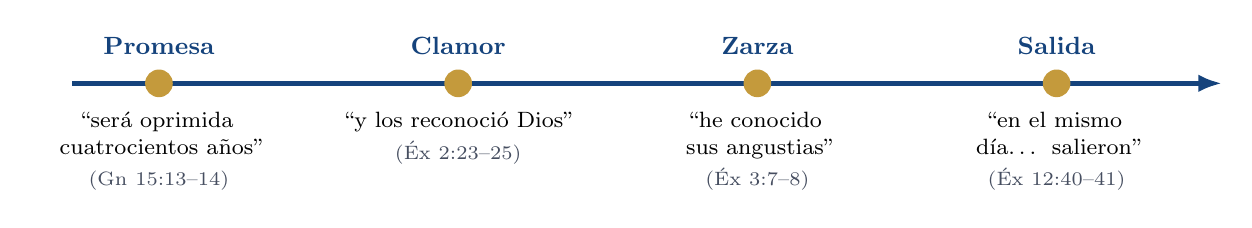
\begin{tikzpicture}
 \draw[line width=1.6pt,azul,-{Latex[length=3mm]}] (0,0) -- (14.6,0);
 \foreach \x/\t/\d/\r in {1.1/{Promesa}/{``será oprimida cuatrocientos años''}/{Gn 15:13--14},
   4.9/{Clamor}/{``y los reconoció Dios''}/{Éx 2:23--25},
   8.7/{Zarza}/{``he conocido sus angustias''}/{Éx 3:7--8},
   12.5/{Salida}/{``en el mismo día\ldots{} salieron''}/{Éx 12:40--41}}{
  \fill[dorado] (\x,0) circle (5pt);
  \node[above=7pt,font=\small\bfseries,text=azul] at (\x,0) {\t};
  \node[below=7pt,text width=3.1cm,align=center,font=\footnotesize] at (\x,0) {\d\\[2pt]{\scriptsize\color{gris}(\r)}};}
\end{tikzpicture}\par
{\footnotesize\color{gris}\textit{Figura 4.} Presciencia, omnisciencia compasiva y cumplimiento en el Éxodo. \textit{Nota.} Elaboración propia.}
\end{center}

Dios conocía el sufrimiento de Israel antes de que empezara (Gn 15) y lo conoció mientras ocurría (Éx 3). Saberlo de antemano no lo hizo indiferente: cuando llegó la hora, oyó, se acordó, miró, conoció y descendió.

\begin{nota}[Precisión]
La elección de este encuentro es propia de la serie y conviene confirmarla. La relación entre los cuatrocientos años de Gn 15:13 y los cuatrocientos treinta de Éx 12:40 se explica de varias maneras (cifra redonda, distintos puntos de partida); Pablo cuenta cuatrocientos treinta años desde la promesa hasta la ley (Gá 3:17).
\end{nota}

%===================================================================
\section{La omnisciencia en el judaísmo}

\subsection{``Todo está previsto, y la libertad está dada''}
La fórmula judía más conocida sobre la presciencia está en la Misná:

\hebverso{הַכֹּל צָפוּי וְהָרְשׁוּת נְתוּנָה \\ וּבְטוֹב הָעוֹלָם נִדּוֹן וְהַכֹּל לְפִי רֹב הַמַּעֲשֶׂה}
\begin{cita}Todo está previsto, y la libertad está dada; el mundo es juzgado con bondad, y todo según la mayoría de las obras.\fuente{(Misná, \emph{Avot} 3:15)}\end{cita}

\begin{filologia}[\emph{Avot} 3:15]
\begin{tabular}{@{}L{3.2cm}L{1.6cm}L{10cm}@{}}
\heb{צָפוּי} \emph{tsafuy} & \heb{צפה} & ``previsto'', ``observado'': la raíz de ``los ojos del \SENOR{} están en todo lugar, \emph{mirando}'' (\heb{צֹפוֹת}, Pr 15:3). \\[2pt]
\heb{הָרְשׁוּת} \emph{harshut} & \heb{רשׁה} & ``el permiso'', ``la autorización'': la libertad de elegir. \\
\end{tabular}
\end{filologia}

El dicho se atribuye a Rabí Aquiba (siglo \textsc{ii}), por el contexto de la Misná. Pone lado a lado lo que la filosofía tiende a separar: presciencia y libertad. No las reconcilia con una teoría; las afirma juntas, como hace Pedro en Hch 2:23.

En otro lugar del mismo tratado, Rabí (Yehudá ha-Nasí) aconseja: ``Sabe qué hay sobre ti: un ojo que ve y un oído que oye (\heb{עַיִן רוֹאָה וְאֹזֶן שׁוֹמַעַת}), y todas tus obras se escriben en un libro'' (\emph{Avot} 2:1). Es la ética del Salmo 139 y del Salmo 56: vivir delante del que ve y lleva registro.

\begin{nota}[Precisión]
Misná según Sefaria, traducción propia. La atribución a Aquiba se deduce del contexto (\emph{Avot} 3:13--15).
\end{nota}

\subsection{Rosh Hashaná: todos pasan delante de él}
La Misná describe el juicio del Año Nuevo con un verso del Salmo 33:

\hebverso{בְּרֹאשׁ הַשָּׁנָה כָּל בָּאֵי הָעוֹלָם עוֹבְרִין לְפָנָיו כִּבְנֵי מָרוֹן}
\begin{cita}En Rosh Hashaná todos los que vienen al mundo pasan delante de él como \emph{benei marón}, como está dicho: ``El formó el corazón de todos ellos; Atento está a todas sus obras'' (Sal 33:15).\fuente{(Misná, \emph{Rosh Hashaná} 1:2)}\end{cita}

La expresión \emph{benei marón} es difícil. El Talmud propone que se refiere a las ovejas que pasan una a una por la puerta estrecha del corral para ser contadas, o a soldados que desfilan en fila (\emph{Rosh Hashaná} 18a). En ambos casos, la imagen es la misma: Dios ve a cada persona individualmente, no a una multitud anónima. El Salmo 33 da la razón: el que formó el corazón conoce las obras.

La liturgia del Año Nuevo desarrolla el tema en la sección llamada \emph{Zijronot} (``Recordaciones''), que confiesa ante Dios: ``No hay olvido delante del trono de tu gloria, ni hay nada escondido ante tus ojos'' (\heb{אֵין שִׁכְחָה לִפְנֵי כִסֵּא כְבוֹדֶךָ}).

\begin{nota}[Precisión]
La explicación de \emph{benei marón} es la del Talmud de Babilonia. El texto de \emph{Zijronot} se toma del majzor tradicional (cf. Elbogen, 1993); conviene cotejarlo con un majzor impreso.
\end{nota}

\subsection{Dios vio justos e impíos antes de crear}
Un midrash sobre la creación del hombre une la presciencia con la misericordia:

\hebverso{רָאָה צַדִּיקִים וּרְשָׁעִים יוֹצְאִים מִמֶּנּוּ}
\begin{cita}Dijo Rabí Berejiá: Cuando el Santo, bendito sea, vino a crear al primer hombre, vio justos e impíos que saldrían de él. Dijo: si lo creo, saldrán impíos de él; si no lo creo, ¿cómo saldrán justos de él? ¿Qué hizo? Apartó de su rostro el camino de los impíos, asoció a sí la medida de la misericordia, y lo creó.\fuente{(\emph{Bereshit Rabá} 8:4)}\end{cita}

El midrash se apoya en el Sal 1:6: ``\SENOR{} conoce el camino de los justos; mas la senda de los malos perecerá''. La presciencia del mal no detuvo la creación: Dios creó sabiendo, y creó con misericordia. El estudio de la misericordia (capítulo 14) mostró que la tradición judía asocia el nombre \SENOR{} a la medida de la misericordia; aquí esa medida se une a la presciencia.

\begin{nota}[Precisión]
Midrash según Sefaria, traducción propia y abreviada. El paralelo con 1 P 1:20 (el Cordero conocido antes de la fundación del mundo, ver más adelante) es una lectura propia.
\end{nota}

\subsection{Maimónides: él y su saber son uno}
Maimónides plantea la pregunta de manera directa en las leyes del arrepentimiento: si Dios sabe todo lo que será, ¿cómo puede el hombre elegir? Su respuesta (\emph{Mishné Torá}, \emph{Hiljot Teshuvá} 5:5) es que Dios no conoce con un saber externo a él, como los hombres, ``que son ellos y su saber dos''; en Dios, él y su saber son uno. Por eso ``no hay fuerza en el hombre para alcanzar'' cómo conoce Dios, como no puede ver su rostro (Éx 33:20). Y cita a Isaías:

\hebverso{כִּי לֹא מַחְשְׁבוֹתַי מַחְשְׁבוֹתֵיכֶם וְלֹא דַרְכֵיכֶם דְּרָכָי}
\begin{cita}Porque mis pensamientos no son vuestros pensamientos, ni vuestros caminos mis caminos, dijo \SENOR{}.\fuente{(Is 55:8)}\end{cita}

Maimónides concluye que el hombre es responsable de sus obras, aunque no pueda comprender cómo se armoniza eso con el conocimiento divino. En la \emph{Guía de perplejos} (III:17--21) trata la providencia, \emph{hashgajá}, la palabra formada a partir del verbo del Sal 33:14. En el siglo \textsc{xiv}, Gersónides sostuvo que Dios conoce a los particulares solo como parte del orden general del mundo; fue una postura minoritaria y muy discutida dentro del judaísmo.

\begin{nota}[Precisión]
\emph{Mishné Torá} según Sefaria, en paráfrasis propia; la postura de Gersónides se menciona como dato histórico.
\end{nota}

\subsection{Rashi, el Talmud y el Targum}
Tres voces más completan la mirada judía. Rashi, como se vio, lee el ``yo lo he conocido'' de Gn 18:19 como \emph{leshón jibá}, expresión de cariño. El Talmud recoge un dicho de Rabí Janina que limita y a la vez confirma la soberanía divina: ``Todo está en manos del Cielo, excepto el temor del Cielo'', con apoyo en Dt 10:12 (``¿qué pide \SENOR{} tu Dios de ti, sino que temas\ldots?''; \emph{Berajot} 33b). Y el Targum arameo del Salmo 139 amplía el v. 4 para que no quede duda: ``tú, \SENOR{}, conoces todos los pensamientos de mi corazón''.

\subsection{Qumrán: el Dios del conocimiento}
Los textos de Qumrán retoman el título del cántico de Ana. La Regla de la Comunidad, en su instrucción sobre los dos espíritus, dice:

\begin{cita}Del Dios del conocimiento procede todo lo que es y lo que será; antes de que existieran estableció todo su designio.\fuente{(1QS III:15)}\end{cita}

La expresión \heb{אל הדעות} (``Dios del conocimiento'') es la de 1 S 2:3. Bakker (2014) ha mostrado que varios textos de Qumrán interpretan ese título del cántico de Ana como una reflexión sobre la presciencia divina, nacida del estudio de la Escritura. Qumrán une así los dos temas de este capítulo: el \emph{El deot} de Ana y el conocimiento de Dios antes de la creación.

\begin{nota}[Precisión]
1QS III:15 se cita según las traducciones de García Martínez (1992) y Vermes (2004), con redacción adaptada; la transcripción hebrea conviene cotejarla en la edición.
\end{nota}

%===================================================================
\section{La omnisciencia en Cristo, leída con Pablo}

\subsection{``¡Oh profundidad!''}
Pablo cierra tres capítulos sobre el lugar de Israel en el plan de Dios (Ro 9--11) no con una explicación, sino con una doxología:

\begin{cita}¡Oh profundidad de las riquezas de la sabiduría y de la ciencia de Dios! ¡Cuán insondables son sus juicios, e inescrutables sus caminos! Porque ¿quién entendió la mente del Señor? ¿O quién fue su consejero? ¿O quién le dio a él primero, para que le fuese recompensado? Porque de él, y por él, y para él, son todas las cosas. A él sea la gloria por los siglos. Amén.\fuente{(Ro 11:33--36)}\end{cita}

\begin{filologia}[Ro 11:33--34]
\begin{tabular}{@{}L{3.2cm}L{1.6cm}L{10cm}@{}}
\grc{γνώσεως θεοῦ} & \grc{γινώσκω} & ``de la ciencia de Dios'': su conocimiento. \\[2pt]
\grc{ἀνεξεραύνητα} & \grc{ἐραυνάω} & ``insondables'': que no se pueden escudriñar. Es el verbo con que el Espíritu ``escudriña'' lo profundo de Dios (1 Co 2:10). \\[2pt]
\grc{ἀνεξιχνίαστοι} & \grc{ἴχνος} & ``inescrutables'': caminos que no dejan huella que se pueda seguir. \\[2pt]
\grc{τίς γὰρ ἔγνω νοῦν κυρίου} & --- & cita de Is 40:13 según la LXX: nadie le enseñó a Dios lo que sabe. \\
\end{tabular}
\end{filologia}

Pablo, el judío formado en las Escrituras, termina su argumento más difícil como termina el Salmo 139: ``Tal conocimiento es demasiado maravilloso para mí; alto es, no lo puedo comprender'' (Sal 139:6). El conocimiento de Dios no es un problema que se resuelve; es una profundidad ante la cual se adora.

\subsection{El que escudriña los corazones}

\begin{cita}Y de igual manera el Espíritu nos ayuda en nuestra debilidad; pues qué hemos de pedir como conviene, no lo sabemos, pero el Espíritu mismo intercede por nosotros con gemidos indecibles. Mas el que escudriña los corazones sabe cuál es la intención del Espíritu, porque conforme a la voluntad de Dios intercede por los santos.\fuente{(Ro 8:26--27)}\end{cita}

``El que escudriña los corazones'' (\grc{ὁ ἐραυνῶν τὰς καρδίας}) es una forma de nombrar a Dios que viene del Antiguo Testamento: ``Yo \SENOR{}, que escudriño la mente, que pruebo el corazón'' (Jer 17:10; cf. 1 S 16:7; Sal 139:1, 23). Pablo la usa para consolar: cuando no sabemos qué pedir, Dios conoce lo que el Espíritu pide en nosotros. La omnisciencia es aquí ayuda para la oración débil.

Dos versos después viene la cadena que comienza en la presciencia:

\begin{cita}Porque a los que antes conoció, también los predestinó para que fuesen hechos conformes a la imagen de su Hijo, para que él sea el primogénito entre muchos hermanos. Y a los que predestinó, a éstos también llamó; y a los que llamó, a éstos también justificó; y a los que justificó, a éstos también glorificó.\fuente{(Ro 8:29--30)}\end{cita}

\begin{center}
\begin{tikzpicture}[font=\small]
 \foreach \i/\x/\t/\g in {1/0/{antes conoció}/{προέγνω}, 2/3.0/{predestinó}/{προώρισεν}, 3/6.0/{llamó}/{ἐκάλεσεν}, 4/9.0/{justificó}/{ἐδικαίωσεν}, 5/12.0/{glorificó}/{ἐδόξασεν}}{
  \node[draw=azul,line width=0.8pt,fill=papiro,rounded corners=3pt,text width=2.3cm,align=center,inner sep=4pt] (n\i) at (\x,0) {\textbf{\t}\\ \grc{\g}};}
 \foreach \a/\b in {1/2,2/3,3/4,4/5}{\draw[dorado,line width=1.2pt,-{Latex}] (n\a) -- (n\b);}
\end{tikzpicture}\par
{\footnotesize\color{gris}\textit{Figura 5.} La cadena de Romanos 8:29--30. \textit{Nota.} Elaboración propia.}
\end{center}

La cadena empieza en la presciencia y termina en la gloria, y no pierde a nadie en el camino: los mismos que fueron conocidos de antemano son los que llegan a ser glorificados. El verbo ``glorificó'' está en pasado, como si ya hubiera ocurrido: lo que Dios conoció antes es tan seguro como lo que ya pasó.

\subsection{``Al cual desde antes conoció'': Israel}

\begin{cita}Digo, pues: ¿Ha desechado Dios a su pueblo? En ninguna manera. Porque también yo soy israelita, de la descendencia de Abraham, de la tribu de Benjamín. No ha desechado Dios a su pueblo, al cual desde antes conoció\ldots{} Así también aun en este tiempo ha quedado un remanente escogido por gracia.\fuente{(Ro 11:1--2, 5)}\end{cita}

Pablo aplica la presciencia a Israel. Su pregunta repite casi palabra por palabra el Salmo 94: ``Porque no abandonará \SENOR{} a su pueblo'' (Sal 94:14; LXX 93:14: \grc{οὐκ ἀπώσεται κύριος τὸν λαὸν αὐτοῦ}). Y el ``desde antes conoció'' recoge el ``conocer'' de Amós 3:2: ``A vosotros solamente he conocido''. La presciencia es una garantía: lo que Dios conoció de antemano no lo desecha.

\begin{nota}[Precisión]
El eco del Sal 94:14 en Ro 11:1--2 es claro en la forma verbal (\grc{ἀπωθέω}); lo señalan comentaristas como Moo (1996).
\end{nota}

\subsection{Ser conocidos antes que conocer}
En las cartas indiscutidas de Pablo, el conocimiento de Dios sobre nosotros es anterior al nuestro y lo hace posible:

\begin{cita}Pero si alguno ama a Dios, es conocido por él.\fuente{(1 Co 8:3)}\end{cita}

\begin{cita}mas ahora, conociendo a Dios, o más bien, siendo conocidos por Dios, ¿cómo es que os volvéis de nuevo a los débiles y pobres rudimentos, a los cuales os queréis volver a esclavizar?\fuente{(Gá 4:9)}\end{cita}

\begin{cita}Ahora vemos por espejo, oscuramente; mas entonces veremos cara a cara. Ahora conozco en parte; pero entonces conoceré como fui conocido.\fuente{(1 Co 13:12)}\end{cita}

\begin{filologia}[1 Co 13:12]
\begin{tabular}{@{}L{3.2cm}L{1.6cm}L{10cm}@{}}
\grc{γινώσκω ἐκ μέρους} & \grc{γινώσκω} & ``conozco en parte'': el conocimiento humano es fragmentario. \\[2pt]
\grc{ἐπιγνώσομαι καθὼς καὶ ἐπεγνώσθην} & \grc{ἐπιγινώσκω} & ``conoceré plenamente como también fui plenamente conocido''. El creyente nunca será omnisciente, pero conocerá al modo en que fue conocido: cara a cara. \\
\end{tabular}
\end{filologia}

Por eso el verso que une esta obra empieza en Dios. Jeremías invita a ``entender y conocer'' al \SENOR{} (Jer 9:24), y Pablo explica que ese conocimiento es respuesta: podemos conocerlo porque él nos conoció primero.

\subsection{En Cristo, todos los tesoros}

\begin{cita}para que sean consolados sus corazones, unidos en amor, hasta alcanzar todas las riquezas de pleno entendimiento, a fin de conocer el misterio de Dios el Padre, y de Cristo, en quien están escondidos todos los tesoros de la sabiduría y del conocimiento.\fuente{(Col 2:2--3)}\end{cita}

El conocimiento infinito de Dios no está repartido en fragmentos: está ``escondido'' en una Persona (\grc{ἐν ᾧ εἰσιν πάντες οἱ θησαυροὶ τῆς σοφίας καὶ γνώσεως ἀπόκρυφοι}). Es la tesis de esta obra: ``en él habita corporalmente toda la plenitud de la Deidad'' (Col 2:9).

\begin{nota}[Precisión]
La autoría paulina de Colosenses se discute; la misma idea aparece en una carta indiscutida: Cristo es ``sabiduría de Dios'' (1 Co 1:24, 30).
\end{nota}

Los evangelios muestran a Jesús ejerciendo ese conocimiento. Vio a Natanael debajo de la higuera antes de que Felipe lo llamara (Jn 1:48). ``No tenía necesidad de que nadie le diese testimonio del hombre, pues él sabía lo que había en el hombre'' (Jn 2:25). Anunció la traición antes de que ocurriera, ``para que cuando suceda, creáis que yo soy'' (Jn 13:19). Y en Apocalipsis, el Cristo resucitado toma para sí la frase que en Jeremías define al \SENOR{}: ``yo soy el que escudriña la mente y el corazón'' (Ap 2:23; cf. Jer 17:10). La omnisciencia es una marca de su deidad.

\begin{nota}[Precisión]
Sobre Mr 13:32 (``de aquel día y de la hora nadie sabe\ldots{} ni el Hijo''), la tradición lo explica por la condición de siervo que el Hijo asumió al hacerse hombre (Flp 2:7); el texto no niega su deidad, sino que describe su humillación.
\end{nota}

\subsection{Pedro: el conocido de antemano}
El apóstol que más usa el vocabulario de la presciencia es Pedro. Su historia muestra por qué.

Antes de la pasión, Jesús le anunció su caída y su restauración: ``Simón, Simón, he aquí Satanás os ha pedido para zarandearos como a trigo; pero yo he rogado por ti, que tu fe no falte; y tú, una vez vuelto, confirma a tus hermanos'' (Lc 22:31--32). Pedro protestó, y Jesús le dijo: ``el gallo no cantará hoy antes que tú niegues tres veces que me conoces'' (22:34). Cuando ocurrió, ``vuelto el Señor, miró a Pedro'' (22:61). Después de la resurrección, a la tercera pregunta, Pedro respondió con la confesión de la omnisciencia: ``Señor, tú lo sabes todo; tú sabes que te amo'' (Jn 21:17).

\begin{center}
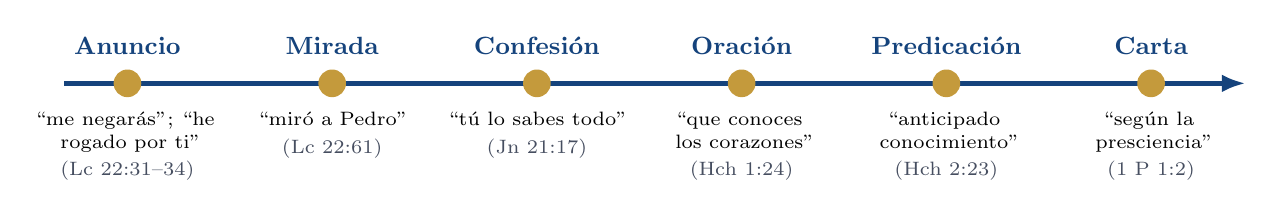
\begin{tikzpicture}
 \draw[line width=1.6pt,azul,-{Latex[length=3mm]}] (0,0) -- (15.0,0);
 \foreach \x/\t/\d/\r in {0.8/{Anuncio}/{``me negarás''; ``he rogado por ti''}/{Lc 22:31--34},
   3.4/{Mirada}/{``miró a Pedro''}/{Lc 22:61},
   6.0/{Confesión}/{``tú lo sabes todo''}/{Jn 21:17},
   8.6/{Oración}/{``que conoces los corazones''}/{Hch 1:24},
   11.2/{Predicación}/{``anticipado conocimiento''}/{Hch 2:23},
   13.8/{Carta}/{``según la presciencia''}/{1 P 1:2}}{
  \fill[dorado] (\x,0) circle (5pt);
  \node[above=7pt,font=\small\bfseries,text=azul] at (\x,0) {\t};
  \node[below=7pt,text width=2.3cm,align=center,font=\scriptsize] at (\x,0) {\d\\[2pt]{\color{gris}(\r)}};}
\end{tikzpicture}\par
{\footnotesize\color{gris}\textit{Figura 6.} Pedro y la presciencia. \textit{Nota.} Elaboración propia.}
\end{center}

En el aposento alto, la oración que Pedro preside llama a Dios \grc{καρδιογνώστης}, ``conocedor de corazones'' (Hch 1:24). En Pentecostés predica la cruz como obra del ``determinado consejo y anticipado conocimiento de Dios'' (Hch 2:23). En el concilio de Jerusalén apela otra vez al \grc{καρδιογνώστης θεός}: ``Dios, que conoce los corazones, les dio testimonio, dándoles el Espíritu Santo lo mismo que a nosotros'' (Hch 15:8). Y en su primera carta saluda a los creyentes como ``elegidos según la presciencia de Dios Padre''. Pedro, que fue conocido de antemano en su caída y en su restauración, es el apóstol de la presciencia.

\begin{nota}[Precisión]
La lectura biográfica que une estos textos es propia de la serie.
\end{nota}

\subsection{Pedro y los Salmos: lo que Dios dijo antes}
Pedro no habla de la presciencia en abstracto. Cada vez que la nombra, la prueba con las Escrituras de Israel, y casi siempre con los Salmos. Para él, que Dios conozca de antemano se demuestra en que Dios \emph{dijo} de antemano. El primer discurso suyo que registra Hechos, antes incluso de Pentecostés, empieza así:

\begin{cita}Varones hermanos, era necesario que se cumpliese la Escritura en que el Espíritu Santo habló antes por boca de David acerca de Judas, que fue guía de los que prendieron a Jesús\ldots{} Porque está escrito en el libro de los Salmos: Sea hecha desierta su habitación, Y no haya quien more en ella; y: Tome otro su oficio.\fuente{(Hch 1:16, 20)}\end{cita}

Pedro cita dos salmos de lamento, el 69 (``Sea su palacio asolado; En sus tiendas no haya morador'', Sal 69:25 [69:26]) y el 109 (``Sean sus días pocos; Tome otro su oficio'', Sal 109:8), y los lee como palabra que el Espíritu ``habló antes'' (\grc{προεῖπεν}). La traición de Judas, que había quebrado a los discípulos, no tomó a Dios por sorpresa. Es la misma lógica de Jesús en Lc 24:44: ``era necesario'' (\grc{ἔδει}) que se cumpliera lo escrito ``en los salmos''.

En Pentecostés, dos versos después de nombrar el ``anticipado conocimiento de Dios'' (Hch 2:23), Pedro cita el Salmo 16, que en hebreo comienza \heb{שִׁוִּיתִי יְהוָה לְנֶגְדִּי תָמִיד}, ``A \SENOR{} he puesto siempre delante de mí'' (Sal 16:8):

\begin{cita}Porque David dice de él: Veía al Señor siempre delante de mí; Porque está a mi diestra, no seré conmovido\ldots{} Porque no dejarás mi alma en el Hades, Ni permitirás que tu Santo vea corrupción\ldots{} Pero siendo profeta, y sabiendo que con juramento Dios le había jurado que de su descendencia, en cuanto a la carne, levantaría al Cristo para que se sentase en su trono, viéndolo antes, habló de la resurrección de Cristo, que su alma no fue dejada en el Hades, ni su carne vio corrupción.\fuente{(Hch 2:25, 27, 30--31)}\end{cita}

\begin{filologia}[Hch 1:16; 2:23, 31]
\begin{tabular}{@{}L{3.2cm}L{1.6cm}L{10cm}@{}}
\grc{ἔδει} & \grc{δεῖ} & ``era necesario'': la necesidad que nace del plan de Dios (cf. Lc 24:44). \\[2pt]
\grc{προεῖπεν} & \grc{προλέγω} & ``habló antes'', ``predijo'': el Espíritu dijo por boca de David lo que vendría. \\[2pt]
\grc{προγνώσει} & \grc{προγινώσκω} & ``anticipado conocimiento'' de Dios (2:23). \\[2pt]
\grc{προϊδὼν} & \grc{προοράω} & ``viéndolo antes'' (2:31): David, como profeta, vio de antemano la resurrección. \\
\end{tabular}
\end{filologia}

El discurso tiene una arquitectura cuidada. En el v. 23 Dios \emph{conoce antes} (\grc{πρόγνωσις}); en el v. 30 David \emph{sabe} por el juramento de Dios (Sal 132:11; 2 S 7:12); en el v. 31 David \emph{ve antes} (\grc{προϊδών}). El profeta ve de antemano porque Dios conoce de antemano y se lo revela. Pedro completa el argumento con el Salmo 110: ``Dijo el Señor a mi Señor: Siéntate a mi diestra'' (Hch 2:34--35; Sal 110:1).

Cuando las autoridades amenazan a los apóstoles, la iglesia ora con el Salmo 2 y llega a la misma conclusión que Pedro en Pentecostés:

\begin{cita}Soberano Señor, tú eres el Dios que hiciste el cielo y la tierra, el mar y todo lo que en ellos hay; que por boca de David tu siervo dijiste: ¿Por qué se amotinan las gentes, Y los pueblos piensan cosas vanas? Se reunieron los reyes de la tierra, Y los príncipes se juntaron en uno Contra el Señor, y contra su Cristo. Porque verdaderamente se unieron en esta ciudad contra tu santo Hijo Jesús, a quien ungiste, Herodes y Poncio Pilato, con los gentiles y el pueblo de Israel, para hacer cuanto tu mano y tu consejo habían antes determinado que sucediera.\fuente{(Hch 4:24--28)}\end{cita}

El ``consejo'' (\grc{βουλή}) que en Hch 2:23 iba unido a la presciencia aparece aquí con su verbo, \grc{προώρισεν}, ``habían antes determinado''. Es el lenguaje del Salmo 33: las naciones traman, pero ``el consejo de \SENOR{} permanecerá'' (Sal 33:10--11). Pink (2020, p. 24) apoya en el decreto del Salmo 2:7 la regla de que la presciencia descansa sobre el propósito de Dios, y no al revés.

Años después, en su primera carta, Pedro explica cómo pudieron los profetas hablar así:

\begin{cita}Los profetas que profetizaron de la gracia destinada a vosotros, inquirieron y diligentemente indagaron acerca de esta salvación, escudriñando qué persona y qué tiempo indicaba el Espíritu de Cristo que estaba en ellos, el cual anunciaba de antemano los sufrimientos de Cristo, y las glorias que vendrían tras ellos.\fuente{(1 P 1:10--11)}\end{cita}

Los profetas ``escudriñaban'' (\grc{ἐραυνῶντες}), el verbo con que la Escritura describe a Dios que escudriña los corazones (Ro 8:27; Ap 2:23); y el Espíritu de Cristo ``anunciaba de antemano'' (\grc{προμαρτυρόμενον}, ``testificaba antes'') lo que vendría. La misma carta que comienza con la presciencia del Padre (1:2) y el Cordero conocido antes de la fundación del mundo (1:20) atribuye la profecía a ese conocimiento previo. Y cuando Pedro exhorta a los creyentes a vivir en paz, cita otro salmo del Dios que ve: ``Porque los ojos del Señor están sobre los justos, Y sus oídos atentos a sus oraciones'' (1 P 3:12; Sal 34:15 [34:16]).

\begin{center}\small\renewcommand{\arraystretch}{1.2}
\begin{tabular}{@{}L{2.4cm}L{2.6cm}L{4.6cm}L{4.8cm}@{}}
\toprule
\textbf{Pedro} & \textbf{Salmo} & \textbf{Texto citado} & \textbf{Qué muestra} \\ \midrule
Hch 1:16--20 & 69:25; 109:8 & ``Tome otro su oficio'' & la traición, dicha antes por el Espíritu \\
Hch 2:25--31 & 16:8--11 & ``no dejarás mi alma en el Hades'' & la resurrección, vista de antemano \\
Hch 2:34--35 & 110:1 & ``Siéntate a mi diestra'' & la exaltación del Mesías \\
Hch 4:11 & 118:22 & ``la piedra reprobada'' & el rechazo, anunciado y vencido \\
Hch 4:25--28 & 2:1--2 & ``¿Por qué se amotinan las gentes?'' & el consejo que había determinado antes \\
1 P 2:7 & 118:22 & ``La piedra que los edificadores desecharon'' & Cristo, precioso para los que creen \\
1 P 3:12 & 34:15--16 & ``los ojos del Señor están sobre los justos'' & la mirada de Dios sobre los suyos \\
\bottomrule
\end{tabular}\par
{\footnotesize\color{gris}\textit{Tabla 11.} Los Salmos en la predicación y las cartas de Pedro. \textit{Nota.} Elaboración propia; numeración española de los salmos.}
\end{center}

La conclusión de Pedro es la de este capítulo. Dios conoce todo, y por eso conoce también lo que vendrá; lo dijo por los profetas y por los salmos, y lo cumplió en Cristo. Pero lo que Dios conoció antes no fueron solo hechos, sino una Persona y un pueblo: ``a éste'' (Hch 2:23), ``el Cordero'' (1 P 1:20), ``los elegidos'' (1 P 1:1--2). La presciencia es la omnisciencia vista desde el amor que la precede.

\begin{nota}[Precisión]
La lectura de los Salmos 69 y 109 como profecía de Judas es la de Pedro en Hechos; en su contexto original son lamentos del justo perseguido. La estructura del discurso de Hch 2 (conocer antes, saber, ver antes) es una observación propia sobre el texto griego.
\end{nota}

\subsection{``Elegidos según la presciencia''}

\begin{cita}Pedro, apóstol de Jesucristo, a los expatriados de la dispersión en el Ponto, Galacia, Capadocia, Asia y Bitinia, elegidos según la presciencia de Dios Padre en santificación del Espíritu, para obedecer y ser rociados con la sangre de Jesucristo: Gracia y paz os sean multiplicadas.\fuente{(1 P 1:1--2)}\end{cita}

\begin{filologia}[1 P 1:1--2]
\begin{tabular}{@{}L{3.6cm}L{1.6cm}L{9.6cm}@{}}
\grc{παρεπιδήμοις διασπορᾶς} & --- & ``expatriados de la dispersión'': \emph{diáspora} es el término de Israel disperso entre las naciones. \\[2pt]
\grc{κατὰ πρόγνωσιν θεοῦ πατρός} & \grc{προγινώσκω} & ``según la presciencia de Dios Padre''. \\[2pt]
\grc{ἐν ἁγιασμῷ πνεύματος} & \grc{ἁγιάζω} & ``en santificación del Espíritu''. \\[2pt]
\grc{ῥαντισμὸν αἵματος Ἰησοῦ Χριστοῦ} & \grc{ῥαντίζω} & ``rociamiento de la sangre de Jesucristo'': evoca la sangre del pacto rociada en el Sinaí (Éx 24:8). \\
\end{tabular}
\end{filologia}

La presciencia es aquí del Padre, que conoce de antemano, y alcanza su fin en la santificación y en la sangre de Jesucristo. Para un pueblo disperso y extranjero, la presciencia dice que no son anónimos: fueron conocidos y amados antes de llegar a ser.

\begin{cita}Entonces Moisés tomó la sangre y roció sobre el pueblo, y dijo: He aquí la sangre del pacto que \SENOR{} ha hecho con vosotros sobre todas estas cosas.\fuente{(Éx 24:8)}\end{cita}

\begin{nota}[Precisión]
Pink (2020, p. 24) entiende ``la dispersión'' como judíos creyentes. Muchos comentaristas la leen en sentido figurado, para iglesias que incluían gentiles, por expresiones como ``vuestra vana manera de vivir, la cual recibisteis de vuestros padres'' (1 P 1:18) y ``lo que agrada a los gentiles'' (4:3).
\end{nota}

\subsection{El Cordero conocido antes de la fundación del mundo}

\begin{cita}sabiendo que fuisteis rescatados de vuestra vana manera de vivir, la cual recibisteis de vuestros padres, no con cosas corruptibles, como oro o plata, sino con la sangre preciosa de Cristo, como de un cordero sin mancha y sin contaminación, ya destinado desde antes de la fundación del mundo, pero manifestado en los postreros tiempos por amor de vosotros.\fuente{(1 P 1:18--20)}\end{cita}

\begin{filologia}[1 P 1:20]
\begin{tabular}{@{}L{3.6cm}L{1.6cm}L{9.6cm}@{}}
\grc{προεγνωσμένου} & \grc{προγινώσκω} & ``conocido de antemano'' (RVR1960: ``ya destinado desde antes''). El objeto de la presciencia es Cristo. \\[2pt]
\grc{πρὸ καταβολῆς κόσμου} & \grc{καταβολή} & ``antes de la fundación del mundo''. \\[2pt]
\grc{φανερωθέντος} & \grc{φανερόω} & ``manifestado'': lo conocido desde la eternidad aparece en la historia. \\
\end{tabular}
\end{filologia}

Este texto recuerda el monte Moriá. Cuando Isaac preguntó dónde estaba el cordero, Abraham respondió:

\hebverso{אֱלֹהִים יִרְאֶה־לּוֹ הַשֶּׂה לְעֹלָה בְּנִי}
\begin{cita}Y respondió Abraham: Dios se proveerá de cordero para el holocausto, hijo mío. E iban juntos.\fuente{(Gn 22:8)}\end{cita}

``Se proveerá'' es \heb{יִרְאֶה} (\emph{yiré}), literalmente ``verá''. Dios ``ve de antemano'' el cordero, y Abraham llama al lugar \heb{יְהוָה יִרְאֶה}, ``el \SENOR{} verá'', ``el \SENOR{} proveerá'' (Gn 22:14). La palabra española ``providencia'' viene del latín \emph{pro-videre}, ``ver antes''. En el lenguaje de la Escritura, el Dios que ve de antemano es el Dios que provee.

\begin{nota}[Precisión]
La conexión entre Gn 22 y 1 P 1:19--20 es una lectura tipológica. La etimología latina de ``providencia'' sirve como ilustración, no como prueba del sentido del hebreo.
\end{nota}

\subsection{La presciencia comunicada}
En su segunda carta, Pedro usa el mismo verbo para los creyentes:

\begin{cita}Así que vosotros, oh amados, sabiéndolo de antemano, guardaos, no sea que arrastrados por el error de los inicuos, caigáis de vuestra firmeza.\fuente{(2 P 3:17)}\end{cita}

\grc{προγινώσκοντες}, ``sabiéndolo de antemano'': los creyentes no son omniscientes, pero han sido avisados por la Palabra de lo que vendrá. Es la forma en que la presciencia de Dios llega a nosotros: como revelación. ``Las cosas secretas pertenecen a \SENOR{} nuestro Dios; mas las reveladas son para nosotros y para nuestros hijos para siempre'' (Dt 29:29 [29:28]).

\begin{nota}[Precisión]
La autoría petrina de 2 Pedro se discute en la investigación; el uso del verbo se apoya también en 1 P 1:20.
\end{nota}

%===================================================================
\section{Aplicación: vivir delante del que todo lo sabe}

\subsection{Un atributo incomunicable}
Solo Dios conoce todo: ``sólo tú conoces el corazón de todos los hijos de los hombres'' (1 R 8:39). El ser humano recibe reflejos de ese saber: el conocimiento revelado (Dt 29:29), el aviso de lo que vendrá (2 P 3:17) y, al final, un conocer ``como fui conocido'' (1 Co 13:12). La respuesta propia del creyente no es saberlo todo, sino vivir delante del que lo sabe todo.

\begin{nota}[Precisión]
Clasificación propuesta: incomunicable. Conviene confirmarla.
\end{nota}

\subsection{Orar los Salmos delante del que sabe}
Los Salmos enseñan la respuesta mejor que cualquier lista, porque la omnisciencia aparece en ellos ya convertida en oración. La primera respuesta es el \destacar{temor santo}. ``Los ojos de \SENOR{} están en todo lugar, mirando a los malos y a los buenos'' (Pr 15:3), y ``todas las cosas están desnudas y abiertas a los ojos de aquel a quien tenemos que dar cuenta'' (He 4:13). Pink (2020, p. 19) lo dice con sencillez: ``¡Qué freno sería para nosotros si meditáramos en ello con más frecuencia!''. El que sabe que es visto vive con integridad aun donde nadie más mira, como el justo del Salmo 17, examinado de noche.

Ese mismo temor se vuelve \destacar{consuelo}. Job no entiende su sufrimiento, pero sabe que ``él conoce mi camino'' (Job 23:10); David huye de Saúl y de los filisteos, pero sus lágrimas están en el odre de Dios (Sal 56:8); el Salmo 147 une las estrellas contadas con las heridas vendadas. Ningún dolor queda sin registro, porque el que cuenta las estrellas cuenta también las huidas.

De allí nace la \destacar{oración confiada}. ``Vuestro Padre sabe de qué cosas tenéis necesidad, antes que vosotros le pidáis'' (Mt 6:8). La oración no informa a Dios; descansa en que él ya sabe, como el salmista que dice: ``delante de ti están todos mis deseos, y mi suspiro no te es oculto'' (Sal 38:9). Y cuando no sabemos qué pedir, el que escudriña los corazones entiende lo que el Espíritu pide por nosotros (Ro 8:26--27).

La omnisciencia pide también \destacar{sinceridad}. Adán se escondió entre los árboles (Gn 3:8); David, al final del Salmo 139, se expone: ``Examíname, oh Dios, y conoce mi corazón'' (139:23). Juan da la razón para no temer ese examen: ``si nuestro corazón nos reprende, mayor que nuestro corazón es Dios, y él sabe todas las cosas'' (1 Jn 3:20). El que conoce el pecado es el mismo que conoce ``nuestra condición'' (Sal 103:14).

Y la presciencia da \destacar{seguridad}. ``Conoce el Señor a los que son suyos'' (2 Ti 2:19). Los que Dios conoció de antemano no se pierden en la cadena que lleva a la gloria (Ro 8:29--30); como Pedro, pueden caer, pero el que los conoció antes también rogó por ellos (Lc 22:32). Pink (2020, p. 19) cierra su capítulo sobre la omnisciencia con esa adoración: Dios ``previó cada una de mis caídas'' y, sin embargo, ``fijó su corazón sobre mí''.

\begin{tcolorbox}[colback=papiro,colframe=dorado,boxrule=1.4pt,arc=3pt]
\centering Dios me conoce entero, y aun así puso su amor en mí antes de que yo existiera. ¿Me escondo de él como Adán, o le pido como David: ``Examíname, oh Dios''?
\end{tcolorbox}

%===================================================================
\section{Síntesis}

\begin{tcolorbox}[colback=papiro,colframe=azul,boxrule=1pt,arc=3pt]
El \SENOR{} es \emph{El deot}, ``el Dios de todo saber'' (1 S 2:3). Conoce lo real y lo posible, el pasado y el futuro, y el corazón, sin aprender ni olvidar (Sal 139; Is 46:10; He 4:13). En hebreo, su conocer es relación: \emph{yadá} es mirar con favor y escoger (Gn 18:19; Am 3:2). Por eso la presciencia es la omnisciencia vuelta amor: Dios conoció de antemano a Cristo (1 P 1:20), a Israel (Ro 11:2) y a los suyos (Ro 8:29; 1 P 1:2), según su propósito (Hch 2:23). Israel lo confesó en los Salmos (el que examina, cuenta las estrellas y ``se humilla a mirar'') y en el Éxodo (``y los reconoció Dios''); el judaísmo lo resumió en ``todo está previsto, y la libertad está dada''. Pablo adoró ante su profundidad (Ro 11:33) y Pedro, conocido de antemano en su caída, lo predicó con los Salmos que el Espíritu ``habló antes'' (Hch 1:16; 2:31). En Cristo están escondidos todos los tesoros del conocimiento (Col 2:3).
\end{tcolorbox}

\begin{center}\small\renewcommand{\arraystretch}{1.3}
\begin{tabular}{@{}L{3.0cm}L{11.4cm}@{}}
\toprule
\textbf{Mirada} & \textbf{Aporte al atributo} \\ \midrule
Hebrea & \emph{yadá}, \emph{jaqar}, \emph{bajan}, \emph{El deot}, \emph{temim deím}; los Salmos 1, 7, 11, 17, 33, 38, 44, 56, 69, 90, 94, 103, 105, 113, 139 y 147; el Éxodo: ``y los reconoció Dios''. \\
Judía & ``Todo está previsto, y la libertad está dada'' (\emph{Avot} 3:15); \emph{Avot} 2:1; Rosh Hashaná; el \emph{Hallel} (\emph{Pesajim} 10:6); \emph{Berajot} 10a; \emph{Meguilá} 31a; \emph{Bereshit Rabá} 8:4; Rashi; Maimónides; 1QS III:15. \\
Teológica & alcance (He 4:13), temor (Nm 32:23), consuelo (Job 23:10), oración (Mt 6:8), saber y decretar (Hch 2:23), presciencia de personas (Ro 8:29; 1 P 1:20); Agustín, Boecio, Charnock, Berkhof, Grudem, Moo. \\
Paulina y petrina & Ro 8:27--30; 11:1--2, 33--36; 1 Co 8:3; 13:12; Gá 4:9; Col 2:3; Hch 1:16--20, 24; 2:23--35; 4:24--28; 15:8; 1 P 1:2, 10--11, 20; 3:12; 2 P 3:17. \\
\bottomrule
\end{tabular}\end{center}

\begin{cita}Mas alábese en esto el que se hubiere de alabar: en entenderme y conocerme, que yo soy \SENOR{}, que hago misericordia, juicio y justicia en la tierra; porque estas cosas quiero, dice \SENOR{}.\fuente{(Jer 9:24 [9:23])}\end{cita}

Conocer a Dios, la gloria que Jeremías propone, es posible porque Dios nos conoció antes. El que todo lo sabe nos llama a conocerlo.

%===================================================================
\section*{Compendio bíblico}
\begin{center}\small\renewcommand{\arraystretch}{1.12}
\begin{tabular}{@{}L{2.2cm}L{5.0cm}|L{2.2cm}L{5.0cm}@{}}
\toprule
Gn 16:13 & ``Tú eres Dios que ve'' & Mt 6:8 & ``vuestro Padre sabe\ldots{} antes que vosotros le pidáis'' \\
Gn 18:19 & ``Porque yo sé que mandará a sus hijos'' & Mt 10:30 & ``vuestros cabellos están todos contados'' \\
Gn 22:8 & ``Dios se proveerá de cordero'' & Lc 24:44 & ``lo que está escrito de mí\ldots{} en los salmos'' \\
Éx 3:7 & ``he conocido sus angustias'' & Jn 2:25 & ``él sabía lo que había en el hombre'' \\
Dt 29:29 & ``Las cosas secretas pertenecen a \SENOR{}'' & Jn 21:17 & ``Señor, tú lo sabes todo'' \\
1 S 2:3 & ``el Dios de todo saber es \SENOR{}'' & Hch 1:16 & ``el Espíritu Santo habló antes por boca de David'' \\
1 S 16:7 & ``\SENOR{} mira el corazón'' & Hch 1:24 & ``que conoces los corazones de todos'' \\
1 R 8:39 & ``sólo tú conoces el corazón'' & Hch 2:23 & ``anticipado conocimiento de Dios'' \\
Job 23:10 & ``Mas él conoce mi camino'' & Hch 2:31 & ``viéndolo antes, habló de la resurrección'' \\
Sal 1:6 & ``\SENOR{} conoce el camino de los justos'' & Hch 4:28 & ``tu consejo habían antes determinado'' \\
Sal 7:9 & ``el Dios justo prueba la mente y el corazón'' & Hch 15:8 & ``Dios, que conoce los corazones'' \\
Sal 11:4 & ``Sus ojos ven, sus párpados examinan'' & Ro 8:27 & ``el que escudriña los corazones'' \\
Sal 17:3 & ``Tú has probado mi corazón'' & Ro 8:29 & ``a los que antes conoció'' \\
Sal 33:11 & ``El consejo de \SENOR{} permanecerá'' & Ro 11:2 & ``al cual desde antes conoció'' \\
\bottomrule
\end{tabular}\par
{\footnotesize\color{gris}\textit{Tabla 12.} Compendio bíblico de la omnisciencia y la presciencia (1 de 2). \textit{Nota.} Textos en la RVR1960.}
\end{center}

\begin{center}\small\renewcommand{\arraystretch}{1.12}
\begin{tabular}{@{}L{2.2cm}L{5.0cm}|L{2.2cm}L{5.0cm}@{}}
\toprule
Sal 33:15 & ``Atento está a todas sus obras'' & Ro 11:33 & ``¡Oh profundidad\ldots!'' \\
Sal 38:9 & ``mi suspiro no te es oculto'' & 1 Co 2:10 & ``el Espíritu todo lo escudriña'' \\
Sal 44:21 & ``él conoce los secretos del corazón'' & 1 Co 8:3 & ``es conocido por él'' \\
Sal 56:8 & ``Pon mis lágrimas en tu redoma'' & 1 Co 13:12 & ``conoceré como fui conocido'' \\
Sal 94:9 & ``El que formó el ojo, ¿No verá?'' & Gá 4:9 & ``siendo conocidos por Dios'' \\
Sal 103:14 & ``él conoce nuestra condición'' & Col 2:3 & ``todos los tesoros\ldots{} del conocimiento'' \\
Sal 113:6 & ``Que se humilla a mirar'' & 2 Ti 2:19 & ``Conoce el Señor a los que son suyos'' \\
Sal 139:1 & ``tú me has examinado y conocido'' & He 4:13 & ``todas las cosas están desnudas y abiertas'' \\
Sal 139:16 & ``Mi embrión vieron tus ojos'' & 1 P 1:2 & ``elegidos según la presciencia'' \\
Sal 147:5 & ``su entendimiento es infinito'' & 1 P 1:11 & ``anunciaba de antemano los sufrimientos de Cristo'' \\
Pr 15:3 & ``Los ojos de \SENOR{} están en todo lugar'' & 1 P 1:20 & ``ya destinado desde antes de la fundación'' \\
Is 46:10 & ``anuncio lo por venir desde el principio'' & 1 P 3:12 & ``los ojos del Señor están sobre los justos'' \\
Jer 1:5 & ``Antes que te formase\ldots{} te conocí'' & 1 Jn 3:20 & ``él sabe todas las cosas'' \\
Jer 17:10 & ``que escudriño la mente'' & Ap 2:23 & ``el que escudriña la mente y el corazón'' \\
\bottomrule
\end{tabular}\par
{\footnotesize\color{gris}\textit{Tabla 12.} Compendio bíblico (2 de 2).}
\end{center}

%===================================================================
\section*{Glosario}
\begin{description}\setlength{\itemsep}{2pt}
\item[\emph{Bajan}] (\heb{בָּחַן}). Probar, como se prueba el metal (Sal 139:23).
\item[\emph{Dáat}] (\heb{דַּעַת}). Conocimiento (Sal 94:10; 139:6).
\item[\emph{El deot}] (\heb{אֵל דֵּעוֹת}). ``Dios de todo saber'' (1 S 2:3); en Qumrán, ``Dios del conocimiento'' (1QS III:15).
\item[\emph{El roí}] (\heb{אֵל רֳאִי}). ``Dios que ve'' (Gn 16:13).
\item[\emph{Gnôsis}] (\grc{γνῶσις}). Conocimiento (Ro 11:33; Col 2:3).
\item[\emph{Golem}] (\heb{גֹּלֶם}). Embrión, masa sin forma (Sal 139:16).
\item[\emph{Hallel}] (\heb{הַלֵּל}). ``Alabanza'': los Salmos 113--118, cantados en las fiestas; el 113 lo abre.
\item[\emph{Hashgajá}] (\heb{הַשְׁגָּחָה}). Providencia, en el hebreo posterior; del verbo \emph{shagaj}, ``mirar con atención'' (Sal 33:14).
\item[\emph{Jaqar}] (\heb{חָקַר}). Examinar a fondo, escudriñar (Sal 139:1, 23).
\item[\emph{Kardiognóstes}] (\grc{καρδιογνώστης}). ``Conocedor de corazones'' (Hch 1:24; 15:8).
\item[\emph{Leshón jibá}] (\heb{לְשׁוֹן חִבָּה}). ``Expresión de cariño'': así lee Rashi el ``conocer'' de Gn 18:19.
\item[\emph{Proeîpen}] (\grc{προεῖπεν}). ``Habló antes'': el Espíritu por boca de David (Hch 1:16).
\item[\emph{Proïdón}] (\grc{προϊδών}). ``Viéndolo antes'': David ante la resurrección (Hch 2:31).
\item[\emph{Progignósko}] (\grc{προγινώσκω}). Conocer de antemano (Ro 8:29; 1 P 1:20).
\item[\emph{Prógnosis}] (\grc{πρόγνωσις}). Presciencia (Hch 2:23; 1 P 1:2).
\item[\emph{Temim deím}] (\heb{תְּמִים דֵּעִים}). ``Perfecto en conocimientos'' (Job 37:16).
\item[\emph{Tevuná}] (\heb{תְּבוּנָה}). Entendimiento (Sal 147:5; Is 40:28).
\item[\emph{Taalumot lev}] (\heb{תַּעֲלֻמוֹת לֵב}). ``Los secretos del corazón'' (Sal 44:21).
\item[\emph{Tsafuy}] (\heb{צָפוּי}). Previsto, observado (\emph{Avot} 3:15).
\item[\emph{Yadá}] (\heb{יָדַע}). Conocer, saber; con Dios como sujeto, a menudo conocer con favor y escoger.
\item[\emph{Yetser}] (\heb{יֵצֶר}). ``Hechura'', ``condición'': ``él conoce nuestra condición'' (Sal 103:14).
\item[\emph{Yiré}] (\heb{יִרְאֶה}). ``Verá'', ``proveerá'' (Gn 22:8, 14).
\item[\emph{Zijronot}] (\heb{זִכְרוֹנוֹת}). ``Recordaciones'': sección de la oración del Año Nuevo judío.
\end{description}

\section*{Referencias}
\refapa{Agustín de Hipona. (s.f.). \emph{La ciudad de Dios} [libro V, caps. 9--10]. (Obra original escrita ca. 413--426)}
\refapa{Bakker, A. (2014). The God of knowledge: Qumran reflections on divine prescience based on 1 Sam 2:3. \emph{Revue de Qumrân, 26}(3), 361--374.}
\refapa{Bauer, W., Danker, F.~W., Arndt, W.~F., \& Gingrich, F.~W. (2000). \emph{A Greek-English lexicon of the New Testament and other early Christian literature} (3.ª ed.). University of Chicago Press.}
\refapa{\emph{Bereshit Rabá} [8:4]. (s.f.). Sefaria. https://www.sefaria.org}
\refapa{Berkhof, L. (1938). \emph{Systematic theology}. Eerdmans.}
\refapa{Boecio. (s.f.). \emph{La consolación de la filosofía} [libro V, prosa 6]. (Obra original escrita ca. 524)}
\refapa{Boyd, G.~A. (2000). \emph{God of the possible: A biblical introduction to the open view of God}. Baker Books.}
\refapa{Carson, D.~A. (2013). \emph{Falacias exegéticas}. Editorial CLIE.}
\refapa{Charnock, S. (1996). \emph{The existence and attributes of God} (Vols. 1--2). Baker Books. (Obra original publicada en 1682)}
\refapa{Elbogen, I. (1993). \emph{Jewish liturgy: A comprehensive history} (R.~P. Scheindlin, Trad.). Jewish Publication Society.}
\refapa{Elliger, K., \& Rudolph, W. (Eds.). (1997). \emph{Biblia Hebraica Stuttgartensia} (5.ª ed.). Deutsche Bibelgesellschaft.}
\refapa{García Martínez, F. (1992). \emph{Textos de Qumrán}. Trotta.}
\refapa{Grudem, W. (2007). \emph{Teología sistemática: Una introducción a la doctrina bíblica}. Editorial Vida.}
\refapa{Koehler, L., \& Baumgartner, W. (2001). \emph{The Hebrew and Aramaic lexicon of the Old Testament} (M.~E.~J. Richardson, Trad.; Ed. de estudio). Brill.}
\refapa{Maimónides. (s.f.). \emph{Mishné Torá: Hiljot Teshuvá} [5:5]. Sefaria. https://www.sefaria.org}
\refapa{\emph{Misná: Avot} [2:1; 3:15]; \emph{Pesajim} [10:6]; \emph{Rosh Hashaná} [1:2]. (s.f.). Sefaria. https://www.sefaria.org}
\refapa{Moo, D.~J. (1996). \emph{The epistle to the Romans}. Eerdmans.}
\refapa{Nestle, E., \& Aland, K. (Eds.). (2012). \emph{Novum Testamentum Graece} (28.ª ed.). Deutsche Bibelgesellschaft.}
\refapa{Olson, R.~E. (2006). \emph{Arminian theology: Myths and realities}. IVP Academic.}
\refapa{Pink, A. W. (2020). \emph{Los atributos de Dios} (E. Rodríguez Cruz, Trad.). Chapel Library. (Obra original publicada en 1930)}
\refapa{Pinnock, C., Rice, R., Sanders, J., Hasker, W., \& Basinger, D. (1994). \emph{The openness of God: A biblical challenge to the traditional understanding of God}. InterVarsity Press.}
\refapa{Rahlfs, A., \& Hanhart, R. (Eds.). (2006). \emph{Septuaginta} (Ed. rev.). Deutsche Bibelgesellschaft.}
\refapa{Ramban. (s.f.). \emph{Comentario a la Torá} [Gn 22:1]. Sefaria. https://www.sefaria.org}
\refapa{Rashi. (s.f.). \emph{Comentario a la Torá} [Gn 16:13; 18:19; 22:12]. Sefaria. https://www.sefaria.org}
\refapa{Rashi. (s.f.). \emph{Comentario a los Salmos} [113:5]. Sefaria. https://www.sefaria.org}
\refapa{Sanders, J.~A. (1965). \emph{The Psalms scroll of Qumrân Cave 11 (11QPs\textsuperscript{a})} (Discoveries in the Judaean Desert IV). Clarendon Press.}
\refapa{\emph{Santa Biblia: Reina-Valera 1960}. (1960). Sociedades Bíblicas en América Latina.}
\refapa{Steinsaltz, A. (Ed.). (2017). \emph{Koren Talmud Bavli: Edición William Davidson} [Berajot 10a, 33b; Meguilá 31a; Rosh Hashaná 18a]. Sefaria. https://www.sefaria.org}
\refapa{Strong, J. (1890). \emph{The exhaustive concordance of the Bible}. Hunt \& Eaton.}
\refapa{\emph{Targum a Salmos} [139:4]. (s.f.). Sefaria. https://www.sefaria.org}
\refapa{\emph{Targum Ónkelos} [Gn 16:13]. (s.f.). Sefaria. https://www.sefaria.org}
\refapa{Vermes, G. (2004). \emph{The complete Dead Sea Scrolls in English} (Ed. rev.). Penguin.}

\end{document}
